\documentclass[conference]{IEEEtran}
\usepackage[utf8]{inputenc}
\usepackage{graphicx}
\usepackage{amsmath}
\usepackage{cite}
\usepackage{url}
\usepackage{hyperref}
\usepackage{algorithm}
\usepackage{algpseudocode}
\usepackage{graphicx}
\usepackage{minted}
\usepackage{fancyvrb}

\title{}

\author{
    \IEEEauthorblockN{Luca Zanolo}
    \IEEEauthorblockA{ \textit{luca.zanolo@studenti.unitn.it}\\
    \textit{University of Trento} \\
    Trento, Italy}
}

\begin{document}

\maketitle

\section{Introduction}
\label{sec:intro}

    This project explores the parallel application of the Hough Transform (HT) for line detection on the high-performance computing (HPC) cluster at the University of Trento.
    
    \subsection{Overview}
        \label{sec:intro_overview}
        The project evaluates various implementations of the HT, beginning with the standard version \cite{HT} and extending to more complex variants such as the Probabilistic Hough Transform (PHT) \cite{PHT} and the Progressive Probabilistic Hough Transform (PPHT) \cite{PPHT}. Each variant is implemented in both a sequential and multiple parallel versions, as summarized by Table \ref{tab:ht_version_parallelization}.
        
        \begin{table}[ht]
        \centering
        \caption{HT versions and parallelization strategy implemented.}
        \label{tab:ht_version_parallelization}
        \begin{tabular}{|c|c|c|c|c|}
        \hline
        \textbf{HT Version} & \textbf{Sequential} & \textbf{MPI} & \textbf{OMP} & \textbf{Hybrid} \\ \hline
        HT     & X & X & X & X  \\ \hline
        PHT    & X & X & X & X  \\ \hline
        PPHT   & X & X & X &   \\ \hline
        \end{tabular}
        \end{table}

        At the code level, the project employs both C++ and Python: C++ is used for developing the large part of the project, while Python handles dataset creation, image conversion and test generation. Key modules utilized include gcc91, OMPi-3.0.0--gcc-9.1.0, mpich-3.2.1--gcc-9.1.0, and python-3.7.2. The parallelization strategies for the HT and certain preprocessing steps leverage Message Passing Interface (MPI) or Open Multiprocessing (OMP) and a hybrid approach combining both MPI and OMP libraries.
        The execution of main program and the python scripts is controlled through the Portable Batch System (PBS) script, which allows for the configuration of different resource allocations to mi program on the HPC Cluster.
        
    \subsection{Report Structure}
    \label{sec:intro_rep_struct}
    
        The report is organized as follow: next section introduces the HT and discusses its theoretical foundation and identifies opportunities for parallelization, avoiding implementation specifics. Subsequent sections present the project in detail: Section \ref{sec:prj_org} makes an overview of the project organization, Section \ref{sec:dataset} covers dataset organization, subsequent sections describe the various HT implementations and last Sections \ref{sec::psanalysis} and \ref{subsec:discussion} present the evaluation results and discuss them.
        
\section{Hough Transformation}
\label{sec:HT}

    The HT is a technique in image analysis for detecting lines, curves and other parametric shapes. By transforming the detection problem from image space to parameter space, it simplifies the complex problem of shape detection into a peak detection task. This project focuses on line detection using various implementations of HT.
    
    \subsection{Hough Transform for Line Detection}
    \label{sec:ht_line_detection}
        The HT converts points in the image space $(x, y)$ to a parameter space $(\rho, \theta)$. Here, $\rho$ is the perpendicular distance from the origin \texttt{O} to the line and $\theta$ is the angle between the x-axis and the line normal. The conversion is governed by:
        \begin{equation}
        \label{eq::ht}
            \rho = x \cos(\theta) + y \sin(\theta)
        \end{equation}
        This equation represents each image point as a sinusoidal curve in the parameter space. Lines in the image correspond to points of intersection of these curves in the parameter space. Figure \ref{fig:ht} illustrates how a line can be represented by a pair $(\rho, \theta)$.
    
        \begin{figure}[htbp]
            \centering
            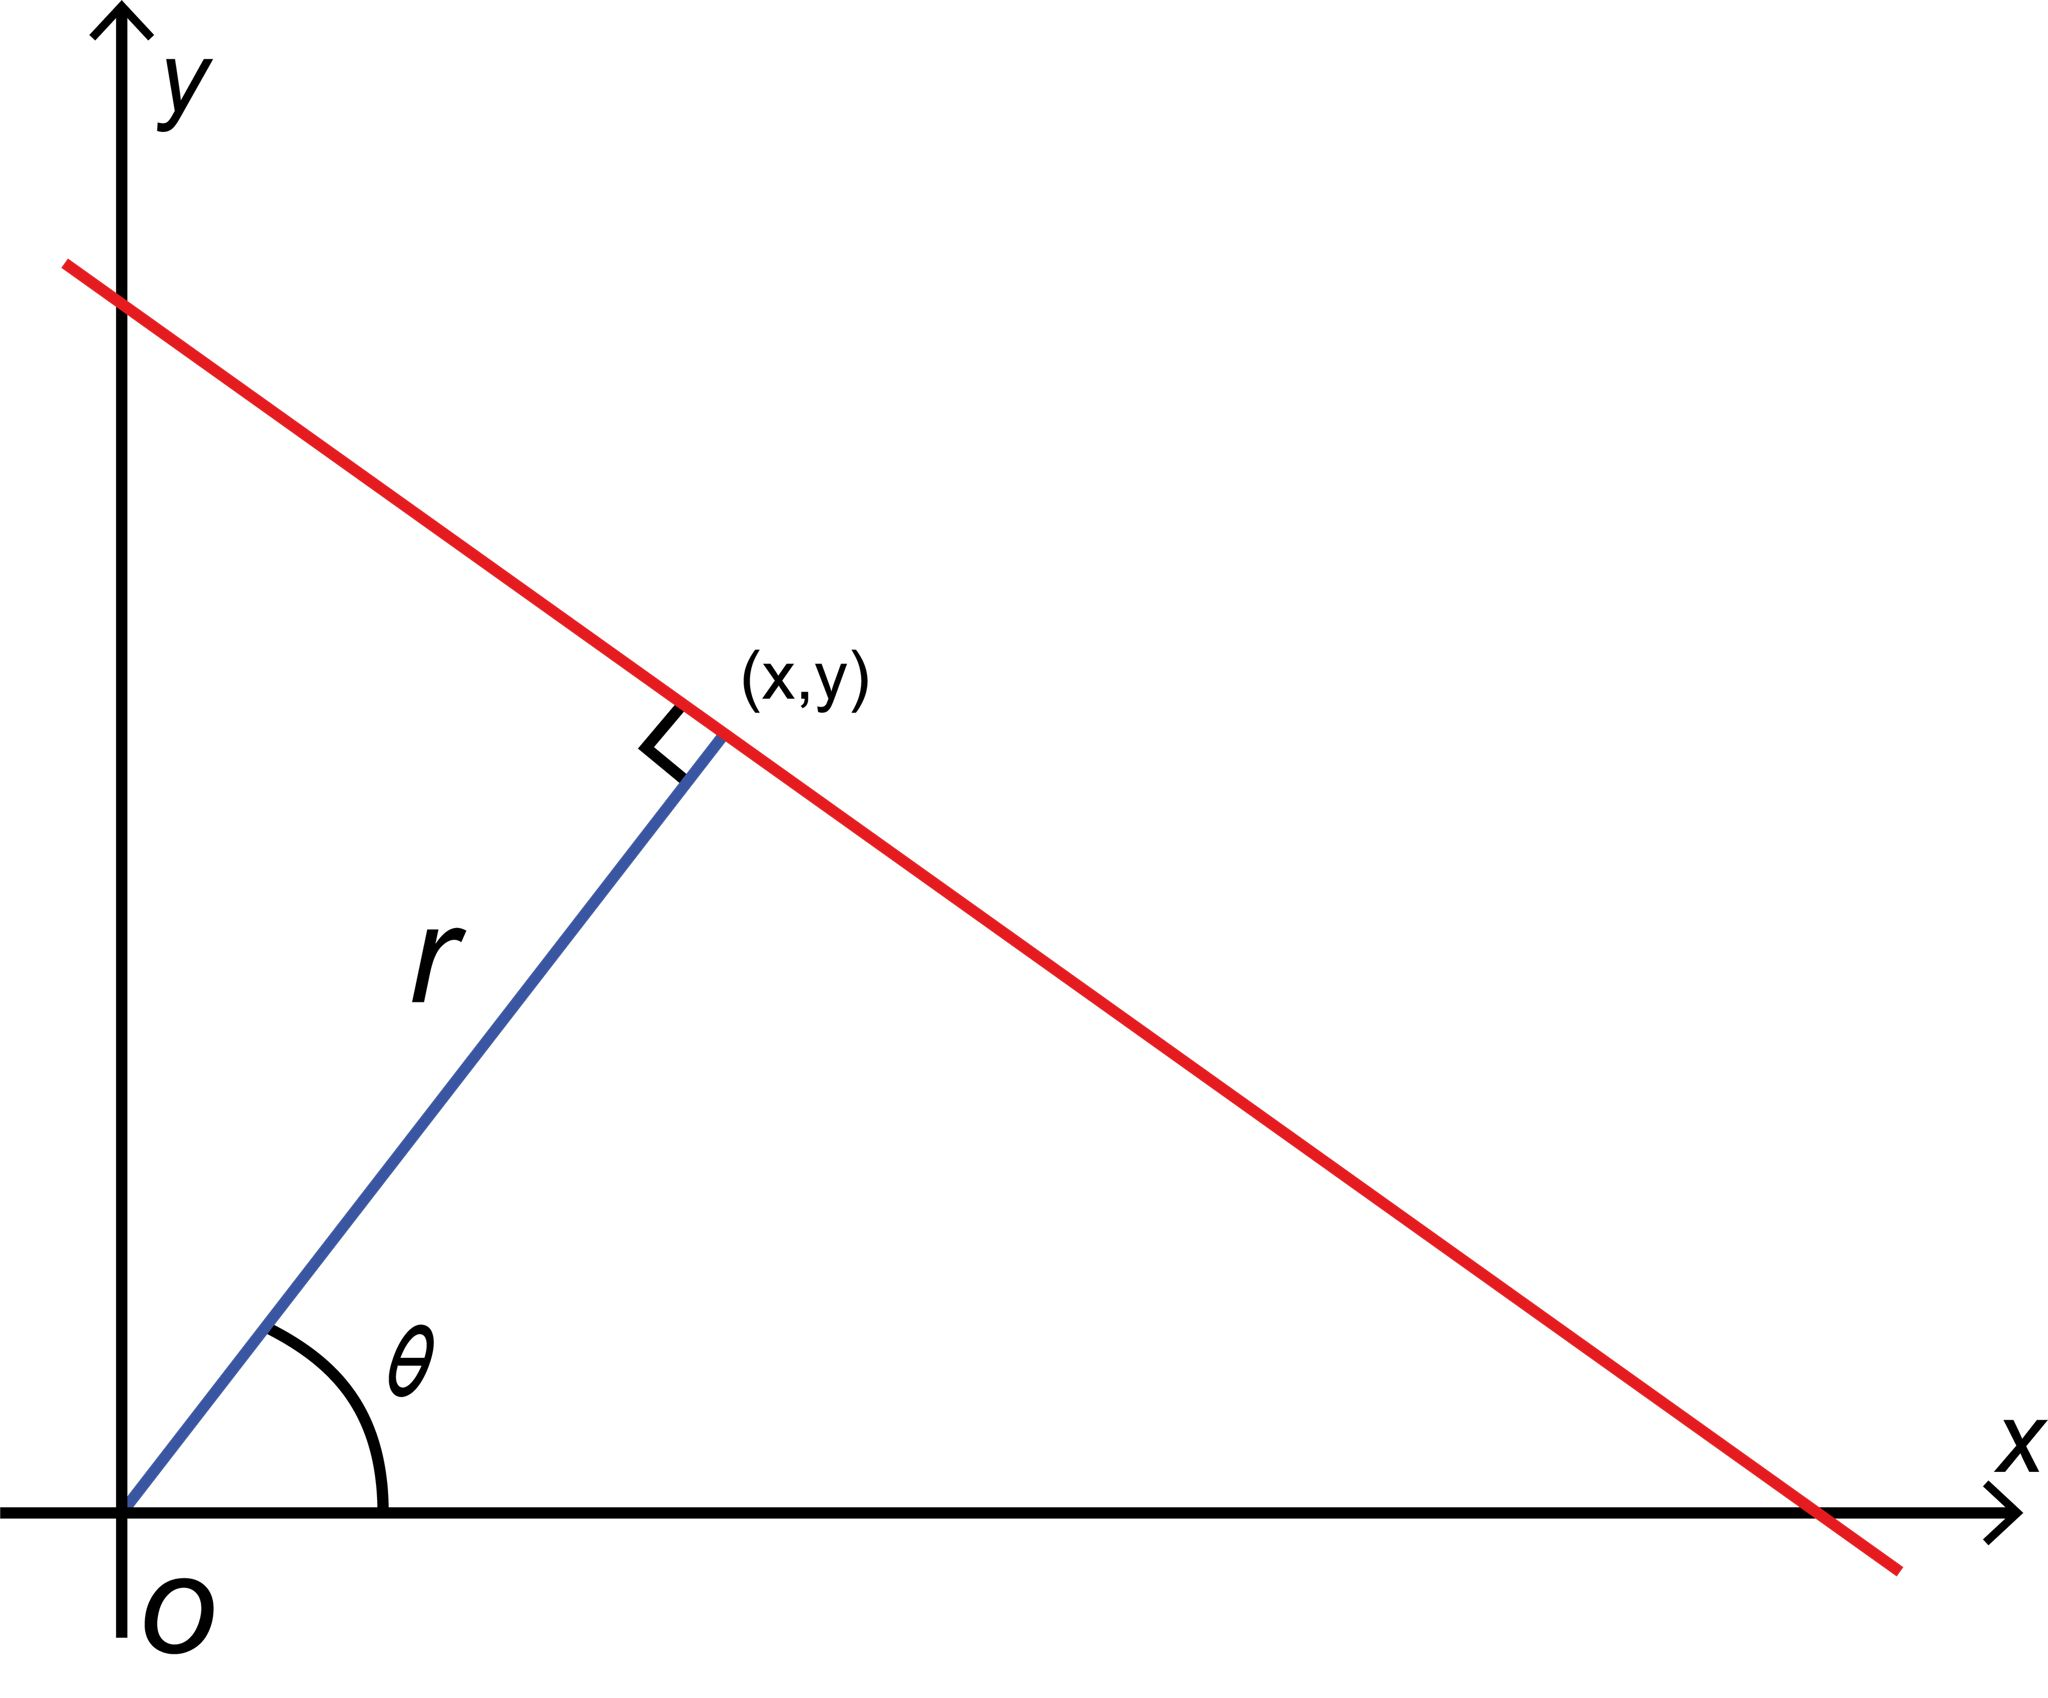
\includegraphics[width=0.4\columnwidth]{ht.jpeg}
            \caption{A line represented with the related $(\rho, \theta)$ parameters highlighted. Original image from \cite{enwiki:1226870376}.}
            \label{fig:ht}
        \end{figure}

    \subsection{Hough Transform Algorithm}
    \label{sec:sht_algorithm}
        The standard HT involves several well-defined steps:
        \begin{enumerate}
            \item \textbf{Edge Detection:} Utilizing edge detection algorithms, such as the Sobel Edge Detection (SED) method, to preprocess the image.
            \item \textbf{Parameter Space Definition:} Employing polar coordinates to define a comprehensive parameter space for line detection.
            \item \textbf{Accumulator Array:} Creating an accumulator array to record votes for each parameter pair $(\rho, \theta)$.
            \item \textbf{Voting:} Allowing edge points in the image to vote for all parameter pairs that could represent lines passing through them.
            \item \textbf{Peak Detection:} Identifying high counts in the accumulator array which suggest the most likely lines in the image space.
        \end{enumerate}

        This algorithm effectively maps edge points from input images into a parametric space where each point is characterized by the pair $(\rho, \theta)$ and an example of the resulting space is illustrated in Figure \ref{fig:ht2}.
        
        \begin{figure}[htbp]
            \centering
            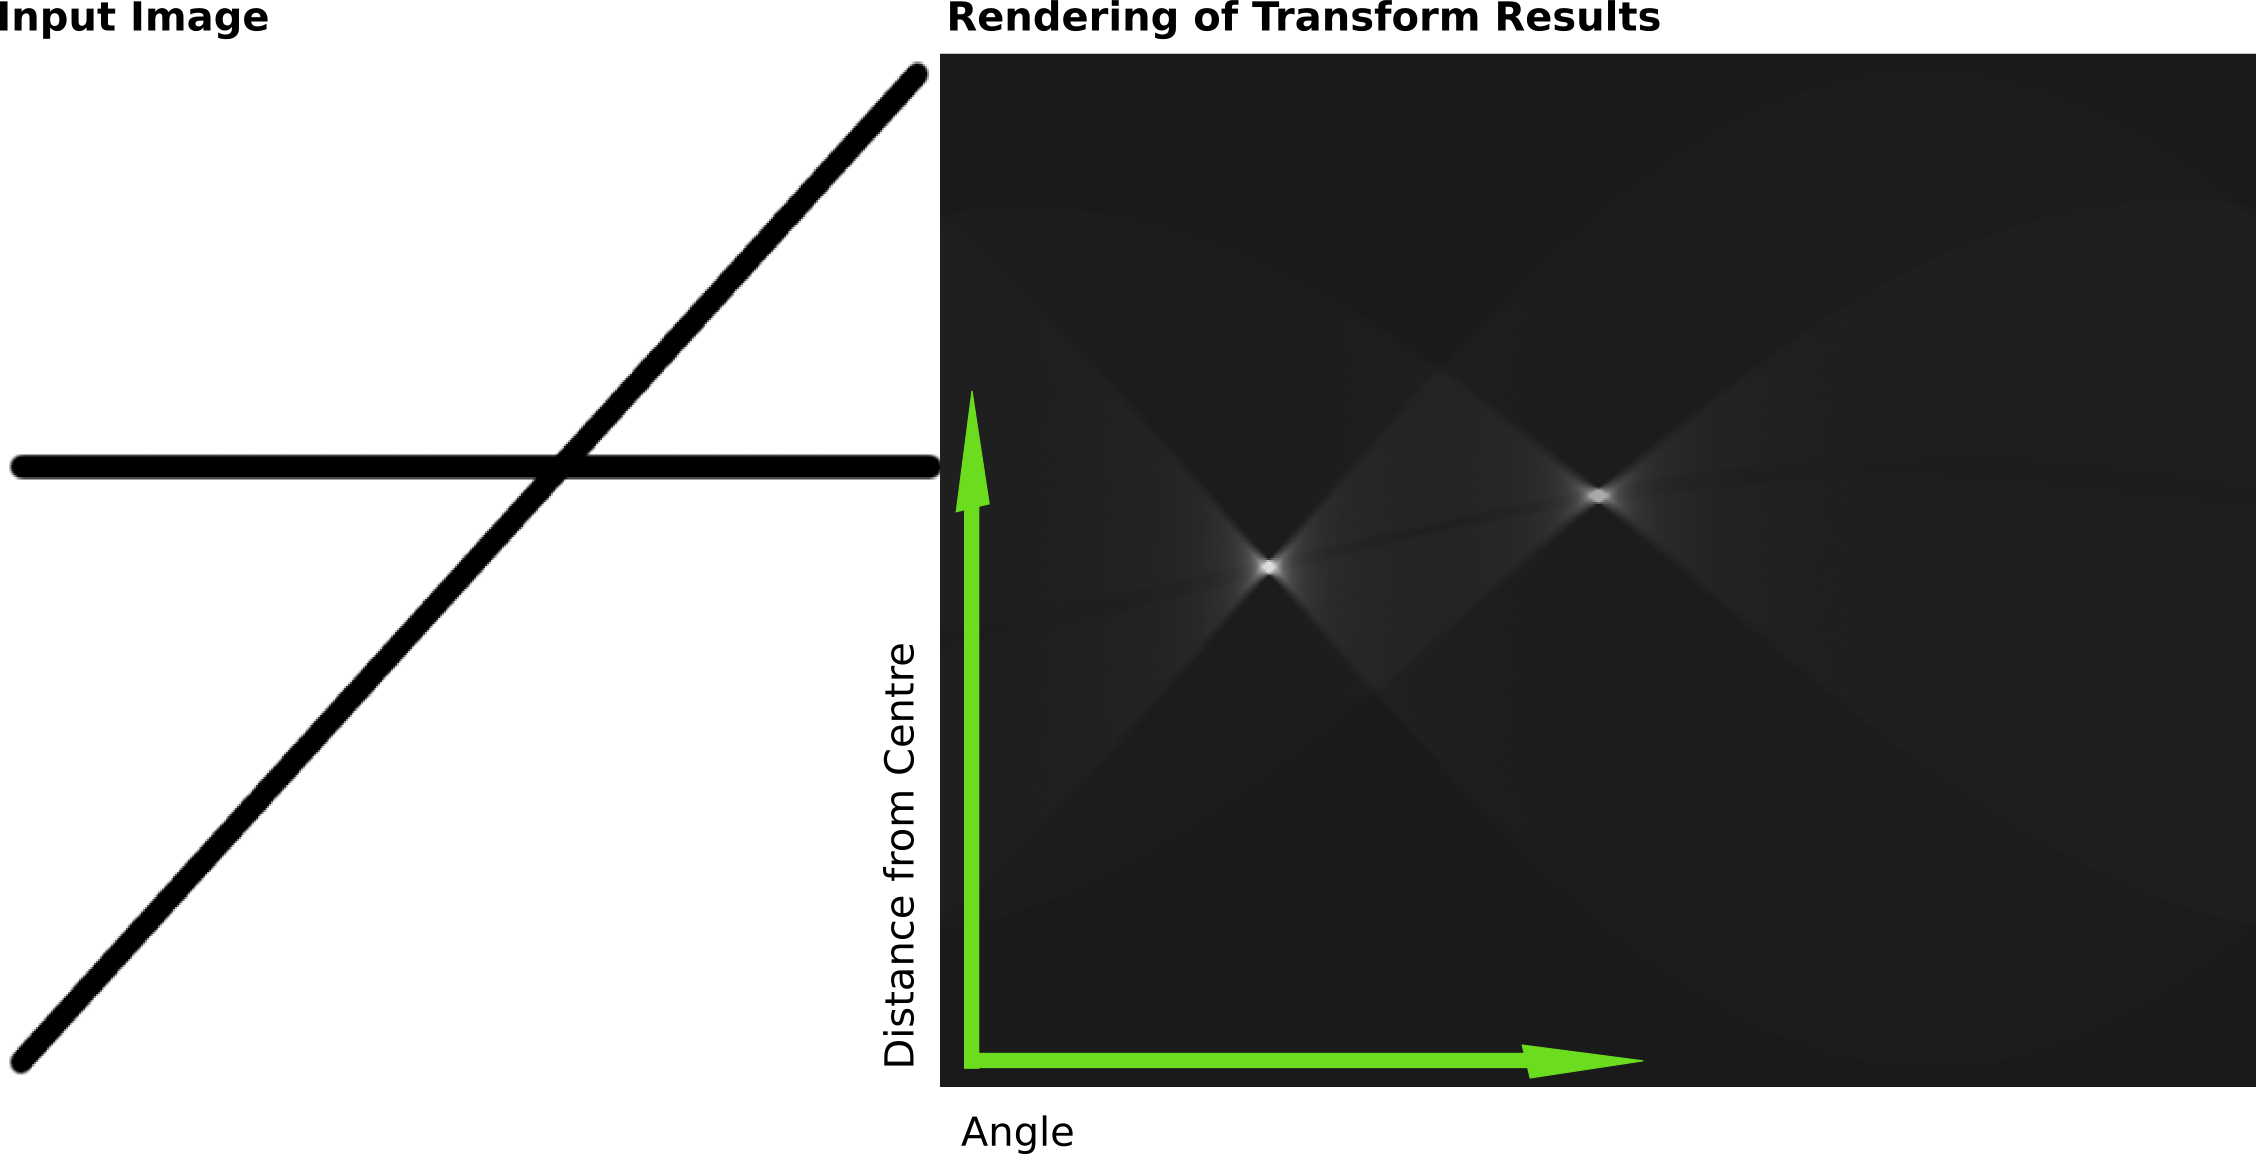
\includegraphics[width=\columnwidth]{ht2.png}
            \caption{Input image and related Hough space where points are represented in terms of $(\rho, \theta)$. Image from \cite{enwiki:1226870376}.}
            \label{fig:ht2}
        \end{figure}

    \subsubsection{Probabilistic Hough Transform}
    \label{sec:pht}
        The PHT modifies the standard HT by randomly sampling edge points rather than using it all. This approach, as detailed in \cite{PHT}, reduces the number of edge points considered speeding up the process while maintaining or improving the quality of the detections. PHT essentially changes the voting mechanism by limiting the number of participating points.
        
    \subsubsection{Progressive Probabilistic Hough Transform}
    \label{sec:ppht}
        The PPHT extends the PHT by dynamically adjusting the threshold for peak detection within the accumulator array. The algorithm proceeds by randomly selecting points for voting, continuously updating the accumulator and testing if the peak values exceed a dynamically computed threshold. When a line is detected, its supporting points reduce their votes and thus also their potential contribution to other segment detections.
                
    \subsection{Parallelization considerations}
    \label{sec:parallel_ht}
        
        This section discusses potential parallelization strategies using both distributed memory programming with MPI and shared memory programming with OMP.
        
        \subsubsection{Distributed Memory Programming with MPI}
    
            Using MPI to parallelize different HT versions involves dividing the image or parameter space among multiple processes, each computing votes in a local accumulator. The primary challenge in this kind of parallelization is managing the communication overhead involved in sharing and combining data from all processes. First bottleneck is rapresented by how the image data are shared among processes and then the second one is rapresented by how the local accumulators are merged. Efficient communication, typically implemented via gathering or reduction operations to a master process will be crucial. Another significant issue is load balancing, which ensures that all processes have an approximately equal amount of work assigned preventing from scenarios where some nodes remain idle, waiting for others to complete their tasks.
    
        \subsubsection{Shared Memory Programming with OMP}
        \label{sec:OMP}
        
            In contrast, parallelizing HT versions using OMP involves parallelizing the loops that iterate through the image pixels and the angle calculations. Each thread can independently update a shared accumulator array with minimal setup, leveraging OMP capabilities to handle thread management and synchronization internally. However, this approach introduces potential data race conditions when multiple threads update the same cell of the accumulator array simultaneously. To address this, synchronization mechanisms such as critical or atomic operations may be employed. While these mechanisms ensure data integrity, they can also introduce significant performance overhead due to the costs associated.
    
        \subsubsection{Hybrid MPI and OMP Approach}
        \label{sec:hybrid_mpi_OMP}
        
        An hybrid approach that combines MPI and OMP can also be employed. Here, MPI could be used to distribute parts of the image across different nodes, reducing the memory demands on any single node. Within each node, OMP can be utilized to further parallelize computations across available CPU cores, optimizing the use of local computational resources. 

\section{Project Organization}
\label{sec:prj_org}

    This section outlines the workflow and structural organization of the project. The high-level workflow is illustrated in Figure \ref{fig:pipeline}.
    
    \begin{figure}[htbp]
        \centering
        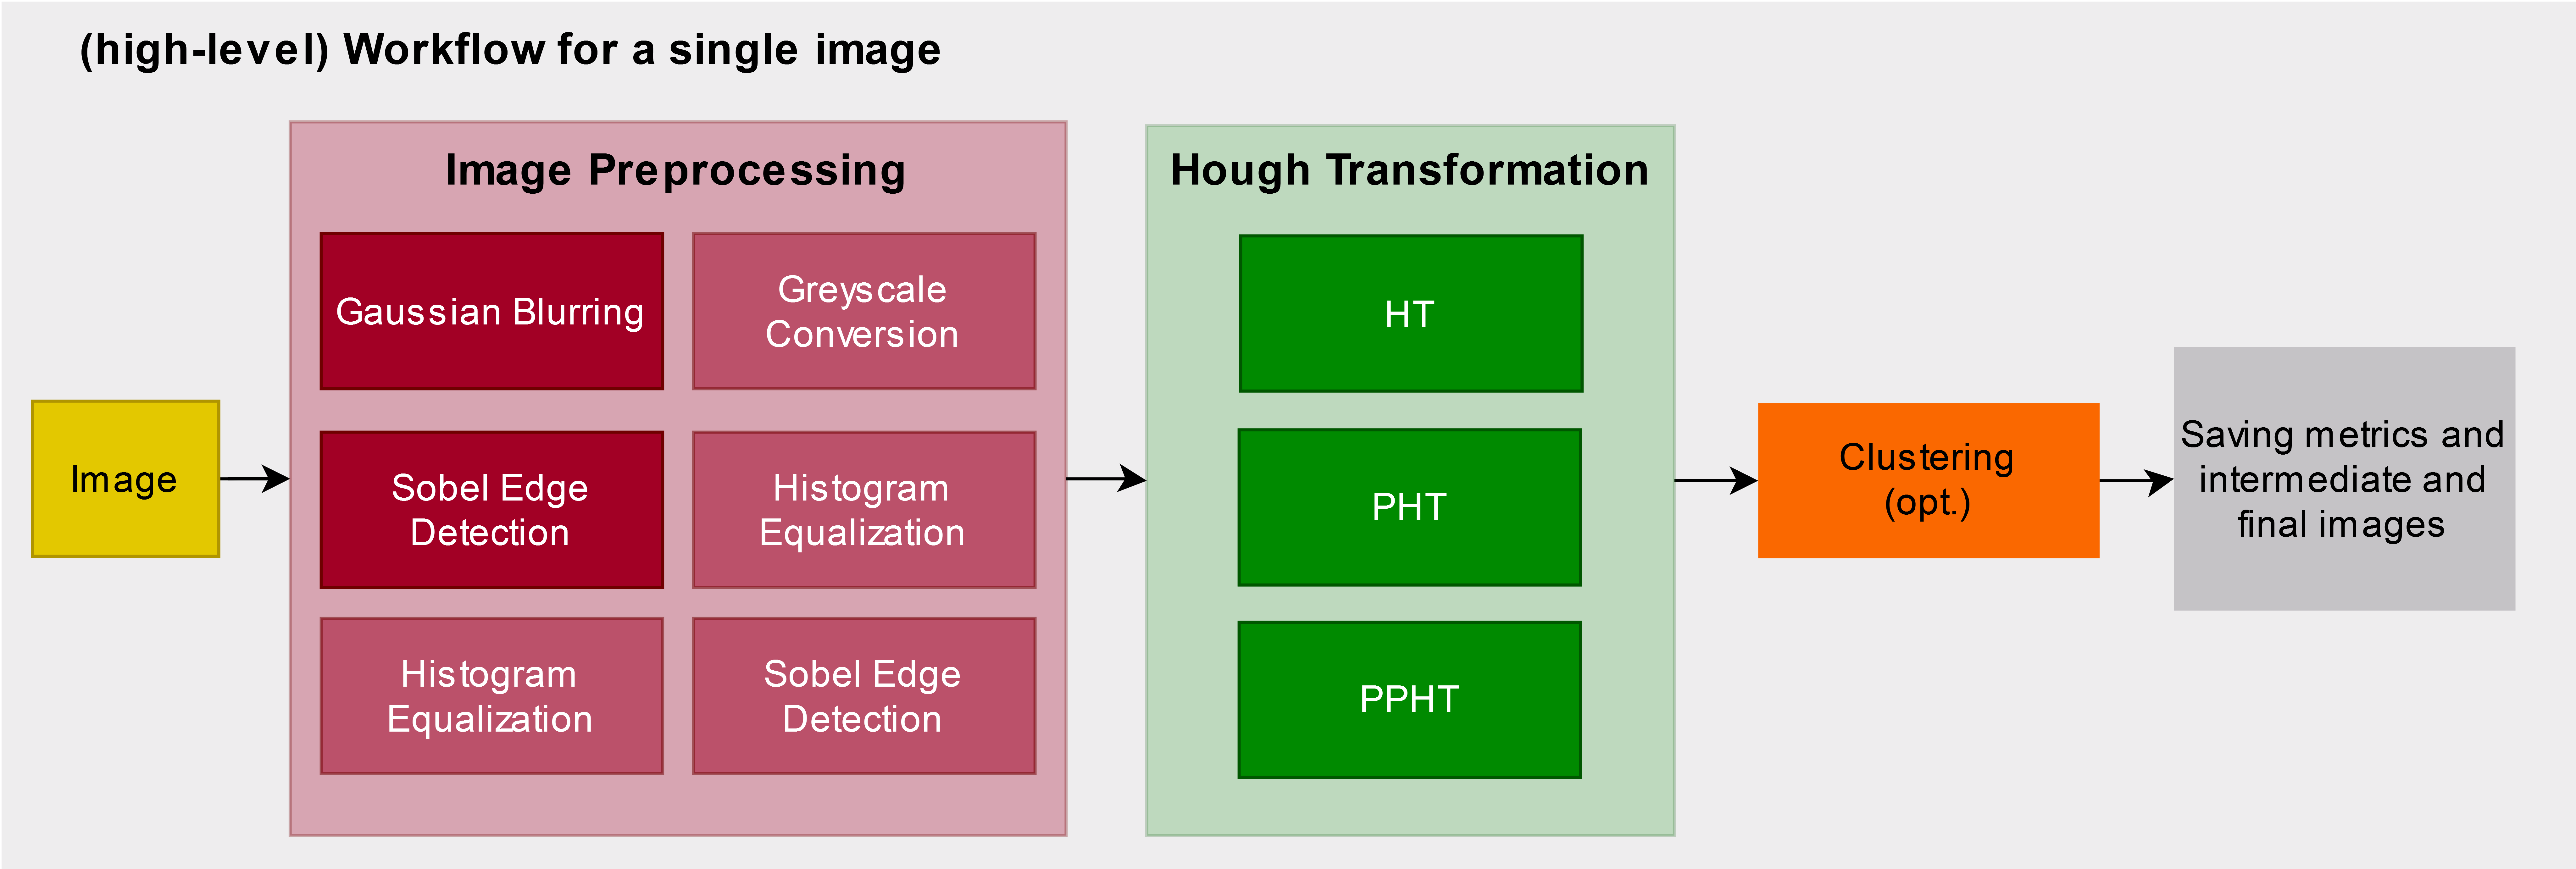
\includegraphics[width=\columnwidth]{hpc4ds-workflow-single-image.png}
        \caption{Project pipeline.}
        \label{fig:pipeline}
    \end{figure}
    
    The project pipeline of Figure \ref{fig:pipeline} begins with reading necessary data and parameters from the file system, facilitated by a parameters file which path is provided as argument to the program. This file allows users to adjust image preprocessing steps, select the HT variant and related parameters, manage post-processing clustering and control file system interactions. The next phase is pre-processing the image, followed by applying the chosen HT version. Afterthat, the HT output may undergo a clustering operation to group lines together. The final step involves evaluating the detection effectiveness and saving the resulting images and metrics.
    
    \begin{figure}[htbp]
        \centering
        \includegraphics[width=0.8\columnwidth]{hpc4ds-package.png}
        \caption{Project package diagram.}
        \label{fig:pkg}
    \end{figure}
    
    Figure \ref{fig:pkg} represents the project package diagram. The main file initiates the program, while the \textit{HoughTransform} (.sh and .exe) objects represent the execution script and executable, respectively. The parameter file, as mentioned, contains specific parameters for different program phases and once built, the program can be executed multiple times with variations in these parameters.
    
    The project folders are organized as follows:
    \begin{enumerate}
        \item \textbf{SRC folder:} Contains all C++ source files. Each component has a .cpp file with the implementation and a .h file with function signatures and descriptions of the operations.
        \item \textbf{Python folder:} Contains Python code for image generation, conversion and test case generation. The image conversion program is also used by the main C++ program when requested in the parameters file.
        \item \textbf{Output folder:} Stores all outputs produced by the project, including images, program messages and \texttt{.err} and \texttt{.out} files saved by PBS after script execution.
        \item \textbf{Dataset folder:} Contains all images used to test the program. Further details on this folder are provided in Section \ref{sec:dataset}.
        \item \textbf{Performance folder:} Holds .csv files documenting all parameters and performance measurements of each program execution.
        \item \textbf{Docs folder:} Contains various theoretical materials related to the project.
    \end{enumerate}

\section{Dataset}
\label{sec:dataset}

    The dataset for this project initially consisted solely of natural environment images. However, to robustly test the program under controlled conditions a Python script was developed to generate synthetic image samples. This generator allows to specify the number of lines, the size of the images, the length of the lines and the number of samples to generate.
    
    \subsection{Synthetic Image Generation}
    \label{subsec:image_generation}
    
        All synthetic samples are stored in a designated folder within the \texttt{dataset} project directory. For each image or batch of images in a specific folder, the generator creates or updates a corresponding .csv file with ground truth data for images segments. Thus, the file contains a row for each line in every image within that specific folder. Each row details:
        \begin{itemize}
            \item The image to which the line belongs.
            \item The start and end points of each line segment.
            \item The coordinates of the projection of each segment to the image borders.
            \item The $\rho$ and $\theta$ parameters for both the segment and its projected line.
        \end{itemize}
    
        These parameters are important for evaluating the algorithm’s performance, as further discussed in Section \ref{sec:psanalysis}.

    \subsection{Synthetic Images for Testing}
    \label{subsec:synthetic_samples}
    
        The synthetic images used to assess the program's performance represent increasing levels of complexity in terms of the number of lines to detect and the image size to process. Table \ref{tab:samples} summarizes the characteristics of these synthetic images and Figure \ref{fig:5k} shows sample \texttt{syn\_img\_5k}.
        
    
        \begin{table}[htbp]
            \centering
            \begin{tabular}{|c|c|c|c|}
            \hline
            \textbf{Sample} & \textbf{Resolution} & \textbf{Lines \#} & \textbf{Lines Length} \\
            \hline
            syn\_img\_5k & 5000x5000 & 100 & 400 \\
            \hline
            syn\_img\_10k & 10000x10000 & 200 & 800 \\ 
            \hline
            syn\_img\_20k & 20000x20000 & 300 & 1200 \\ 
            \hline
            \end{tabular}
            \caption{Predefined synthetic images used for testing different versions of the HT. Resolution and lines length are expressed in pixels.}
            \label{tab:samples}
        \end{table}
    
        \begin{figure}[htbp]
            \centering
            
\includegraphics[width=0.8\columnwidth]{syn_img_5k-3-binary_conversion.jpg}
            \caption{Sample image \texttt{syn\_img\_5k}. The image was altered to make the segments more evident.}
            \label{fig:5k}
        \end{figure}
        
    \subsection{Random Samples}
    \label{subsec:random_samples}
    
        The dataset also contains random samples, created and downloaded from Google Earth, for which ground truth data are not available. In these cases, the results can be visually inspected in the \texttt{output} folder, where the original images are saved with detected lines superimposed on them. This method allows for a qualitative assessment of the HT implementations effectiveness in real-world scenarios, but is not suitable for structured testing of the program's performance.
    
\section{Image Pre-processing}
\label{sec:image_preprocessing}

    Starting with this section the report will describe in details each part of my implementation, following the program workflow presented in Section \ref{sec:prj_org}.
    
    The preprocessing steps available to users are selected through the parameters file to manipulate the image appropriately before line detection. The first and mandatory step is converting the image to grayscale, which simplifies the image data to a single luminance channel, making subsequent processing steps computationally less intensive.
    
    Additional optional image preprocessing steps include:
    \begin{itemize}
        \item \textbf{Gaussian Blurring:} this step blurs the image to reduce noise using a square kernel whose size and $\sigma$ are controlled by parameters. This is particularly useful for real-world images to enhance edge detection efficacy.
        \item \textbf{Histogram Equalization:} this step adjusts the image's contrast, improving the visibility of features across varied lighting conditions.
        \item \textbf{Sobel Edge Detection:} This step, applied before executing the HT, especially the PPHT, uses the Sobel operator to highlight edges in the image, emphasizing areas with high spatial frequency which correspond to edges.
        \item \textbf{Binary Conversion:} The \texttt{toBinary} function is used post-edge detection to convert all pixel values greater than zero to 1, effectively segmenting the image into binary edge and non-edge regions.
    \end{itemize}
    
    \subsection{Parallelization}
    \label{sec:parallelization}
    
        The Gaussian blurring and Sobel edge detection steps, being computationally intensive, have parallel implementations using OMP. This choice avoids the overhead associated with managing data sharing constraints that would arise with MPI.
        
        \textbf{Details on Parallelizing Gaussian Blurring:}
        The parallel version of Gaussian blurring uses OMP to divide the image into blocks, with each block being processed by a separate thread. This division is particularly beneficial when dealing with large images, as it allows the workload to be distributed across multiple cores. Here's how the parallel implementation works:
        
        \begin{itemize}
            \item \textbf{Kernel Sharing:} All threads share a single Gaussian kernel, reducing memory overhead.
            \item \textbf{Image Partitioning:} The image is divided into horizontal strips, with each thread processing one strip.
            \item \textbf{Boundary Handling:} Special care is taken at the boundaries of each strip to ensure that the kernel application does not read uninitialized memory. This is managed by extending the region each thread processes at the borders by the radius of the kernel, though only the central part of the processed region is written back to the output image.
        \end{itemize}
        
    \subsection{Details on Parallelizing Sobel Edge Detection}
    \label{sec:parallel_sobel}
    
        Sobel edge detection, in its sequential form, involves iterating over each pixel (excluding the image border) and applying the Sobel operator to calculate the gradient magnitude. This operation is computational intensive due to the need to access multiple neighboring pixels for each calculation. When parallelized each thread computes the edge detection for a part of the image, similar to the Gaussian blur, After processing, threads synchronize to merge their results into the final output image.
        
        Tests for these two steps were performed with an image downloaded from Google Earth, with a resolution of 8192x4576 pixel, shown in Figure \ref{fig:sat_gb_sed}. The timing of the execution are summarized in Table \ref{tab:preprocessing_time}. Both Gaussian blurring and Sobel edge detection benefit significantly from parallelization, particularly in terms of reduced processing time.

        \begin{table}[htbp]
            \centering
            \begin{tabular}{|c|c|c|c|c|c|}
            \hline
            \textbf{Cores} & 1 (Seq.) & 2 & 4 & 8 & 16\\
            \hline
            \textbf{Time taken} & 52.48s & 28.07s & 14.93s & 9.10s & 5.6s \\
            \hline
            \end{tabular}
            \caption{Preprocessing times averaged on two identical run of the program. Test made are: sequential with 1 core and then parallel with 2,4 and 8 cores available for OMP. Times are taken for the preprocessing of Image \ref{fig:sat_gb_sed}.}
            \label{tab:preprocessing_time}
        \end{table}

        \begin{figure}[htbp]
            \centering
            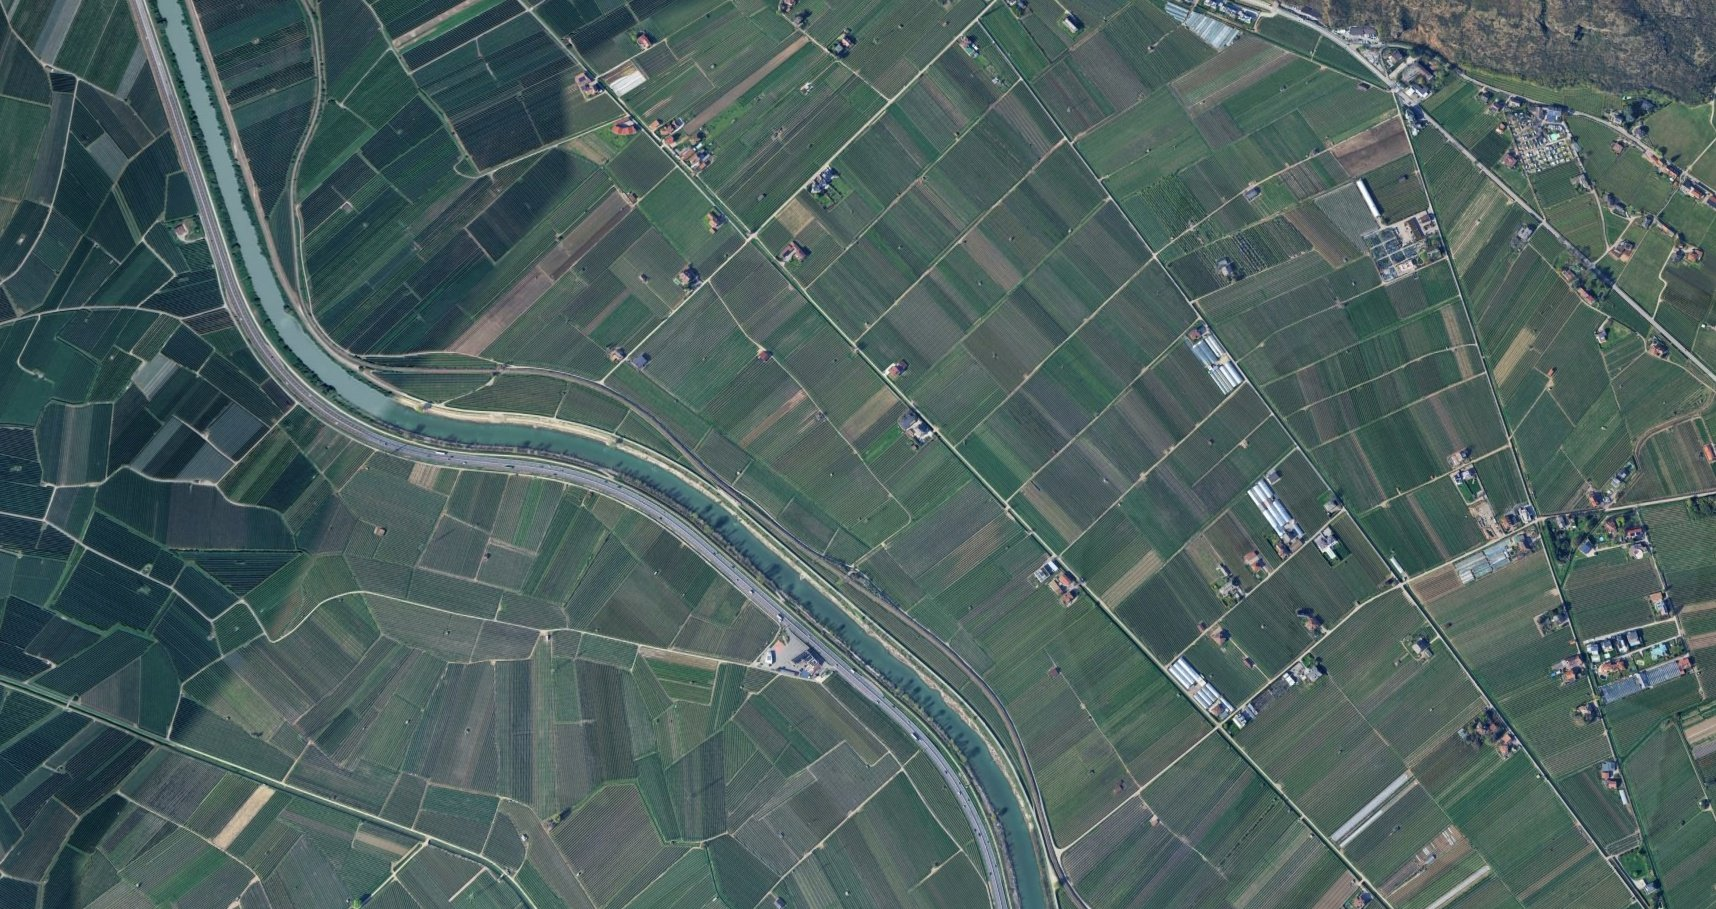
\includegraphics[width=0.9\columnwidth]{sat_img_low_res.jpg}
            \caption{Sample image used to evaluate the Gaussin Blurring and SED parallelization.}
            \label{fig:sat_gb_sed}
        \end{figure}

\section{Implementation of the HT and PHT}
\label{sec:ht_pht_impl}
    
    Both the HT and the PHT are implemented through a unified function, \texttt{HT\_PHT}. This function allows for flexible operation based on specified parameters and encapsulates the process of transforming image space into Hough space, where line detection is achieved by identifying peaks.

    \subsection{Function Overview}
    \label{subsec:function_overview}
        
        The function \texttt{HT\_PHT} initializes by parsing the following parameters from the configuration file: the operational mode (HT or PHT), theta resolution, sampling rate for PHT and the vote threshold necessary for line detection.

    \subsection{Core Processing}
    \label{subsec:core_processing}

        Afterthat, the core processing involves the following key steps:
    
        \begin{enumerate}
            \item \textbf{Point Collection:} The function iterates over image pixels to collect edge points, highlighted using SED method. In PHT mode, points are probabilistically sampled based on the specified rate.
            \item \textbf{Cosine and Sine Precomputation:} Cosine and sine values for each theta value are precomputed to enhance efficiency.
            \item \textbf{Voting Mechanism:} Each selected point casts votes in Hough space for every possible theta angle, transforming its $(x, y)$ coordinates into $(\rho, \theta)$ parameters, using the equation \ref{eq::ht}.
            \item \textbf{Accumulator Array:} This array contains votes across discretized $(\rho, \theta)$ values, with each point potentially contributing to multiple line detections.
        \end{enumerate}

        In all implementations of the HT, operations such as \textbf{Point Collection} and \textbf{Cosine and Sine Precomputation} are performed at the beginning. This sequence facilitates parallelization by isolating the edge points before the voting process. By exclusively distributing edge points, the approach facilitate data transfer and computational load distribution across processes.
        
    \subsection{Line Detection}
    \label{subsec:line_detection}

        Upon populating the accumulator, the next phase of the function identifies entries exceeding the vote threshold as potential lines:
        \begin{enumerate}
            \item Each valid entry's $\rho$ and $\theta$ indices are translated into geometric parameters.
            \item Line endpoints are calculated and mapped from parameter space back to image coordinates.
            \item Detected lines are stored as segments, defined by their endpoints along the image borders, and also the original $(\rho, \theta)$ parameters are saved.
        \end{enumerate}

        These line projections to image borders will be compared against ground truth data, detailed further in Section \ref{sec::psanalysis}.

\section{Parallelization of the Hough Transform}
\label{sec:parallel_ht}

    This section outlines the parallelization strategies used in implementing the HT using MPI, OMP and an hybrid approach, highlighting key aspects of data handling and synchronization.
    
    \subsection{MPI Parallelization}
    \label{subsec:mpi_parallelization}
    
        \subsubsection{Broadcasting Data}
            The MPI approach (and the hybrid approach) begins with the sharing of parameters. Since the parameter file is specified with a path, process 0 reads it from the file system and then broadcasts the content. This initial step is performed in \texttt{main.cpp}, while all subsequent communications are handled within the HT functions.
            
            Following parameter sharing, all processors must align on the image dimensions to ensure that calculations related to pixel positions and transformations into Hough space are consistent. This is achieved using \texttt{MPI\_Bcast} to share the image width and height among all processes.
        
        \subsubsection{Scattering Edge Points}
            The next step is the image's edge pixels distribution among processors. Initially, the image was split into equal stripes, shared among processes. But this approach presents the problem of the potential uneven distribution of workload, as some image parts might have significantly more edge points than others, potentially leaving some processors idle. Instead, the adopted solution involves sampling the edge points only on process 0, applying probabilistic sampling if necessary. Subsequently, from process 0, these edge points are distributed among all processes to guarantee a more balanced workload. \texttt{MPI\_Scatterv} is used for this purpose, as it allows the distribution of unequal chunks of data, its usage is detailed in Algorithm \ref{alg::ht_pht_mpi_scatterv}.
            
            \begin{algorithm}
                \caption{Distribute edge points using MPI\_Scatterv}
                \label{alg::ht_pht_mpi_scatterv}
                \begin{algorithmic}[1]
                    \State \textbf{Parameters:}
                    \State \hspace{\algorithmicindent} counts - array containing the number of elements to send to each process
                    \State \hspace{\algorithmicindent} displs - array specifying the displacement relative to edgePoints from which to take the outgoing data
                    \State \hspace{\algorithmicindent} MPI\_INT - datatype of the elements in edgePoints
                    \State \hspace{\algorithmicindent} rank - rank of the receiving process
                    \State \hspace{\algorithmicindent} MPI\_COMM\_WORLD - communicator
                    \State \textbf{Output:} Local edge points.
                    \Procedure{MPI\_Scatterv}{}
                        \State MPI\_Scatterv(\Call{data}{edgePoints}, 
                        \Call{data}{counts}, \Call{data}{displs}, 
                        MPI\_INT, \Call{data}{localEdgePoints}, 
                        counts[rank], MPI\_INT, 0, MPI\_COMM\_WORLD)
                    \EndProcedure
                \end{algorithmic}
            \end{algorithm}


        \subsubsection{Reducing Results}
        \label{subsubsec:reducing_results}

            Following the scattering of edge points, each processor continues its execution by computing a local accumulator based on its assigned points. The subsequent step is to integrate local accumulators into a global accumulator that represents the global result. This is accomplished using the \texttt{MPI\_Reduce} function consolidating all the local accumulators into a single global accumulator at process 0. The details of this MPI operation are specified in Algorithm \ref{alg::ht_pht_mpi_reduce}. 
        
            To streamline communication, accumulators are flattened into a single-dimensional array during the HT in all MPI implementations. Once the global accumulator is assembled on process 0, for clarity and ease of segment extraction, it is converted back to a 2D vector.
            
            \begin{algorithm}
            \caption{Reduce local accumulators to a global accumulator using MPI\_Reduce}
            \label{alg::ht_pht_mpi_reduce}
            \begin{algorithmic}[1]
            \State \textbf{parameters:}
            \State \hspace{\algorithmicindent} localAccumulator.size() -- number of elements in the local accumulator
            \State \hspace{\algorithmicindent} MPI\_SUM -- operation to be applied (sum)
            \State \hspace{\algorithmicindent} 0 -- root process
            \State \textbf{Output:} Flatten global accumulator
            \Procedure{MPI\_Reduce}{}
                \State MPI\_Reduce(\Call{data}{localAccumulator}, \Call{data}{globalAccumulatorFlatten}, 
                \Call{size}{localAccumulator}, MPI\_INT, MPI\_SUM, 0, MPI\_COMM\_WORLD)
            \EndProcedure
            \end{algorithmic}
            \end{algorithm}

        \subsubsection{Segment Detection on the Root Process}
        
            The final step of segment detection is performed only on process 0. Alternative method involving \texttt{MPI\_AllReduce} to distribute global accumulator and \texttt{MPI\_Gather} to have all segments on process 0 were tested to allow each process to participate in segment detection by distributing the rho ranges. However, due to the overhead associated with these additional synchronization steps, this method was deemed less efficient. Consequently, segment detection is mantained centralized to minimize complexity and synchronization overhead.
            
    \subsection{OMP Parallelization}
    \label{subsec:OMP_parallelization}
    
        OMP is employed to leverage thread level parallelism with a shared memory, thus the bottleneck of sharing image data among processes doesn't exists. Instead the challenges in this kind of parallelization reside more on managing correctly the access to shared resources, such as the accumulator.
        
        \subsubsection{Parallel for loop for detecting edge point}
        \label{sec::plde}
    
            The initial stage in the OMP implementation involves the parallel computation of sine and cosine values for each angle $\theta$ and this is achieved using a \#pragma parallel for loop. Following this, the edge points detection and their probabilistic sampling (if required) are also parallelized. The details of this implementation are outlined in Algorithm \ref{alg::ht_pht_omp_point_collection}, which shows how each thread independently processes the image to identify edge points in parallel.
            
            \begin{algorithm}
            \caption{Parallel point collection in an image}
            \label{alg::ht_pht_omp_point_collection}
            \begin{algorithmic}[1]        
            \State \textbf{parameters:}
            \State \hspace{\algorithmicindent} Image width and height.
            \State \hspace{\algorithmicindent} Total points in the image.
            \State \textbf{Output:} Edge points.
            \Procedure{Parallel Point Collection}{}
                \State \#pragma omp parallel num\_threads(numThreads)
                \State \#pragma omp for collapse(2) reduction(+:totalPoints)
                \For{$y = 0$ to $height-1$}
                    \For{$x = 0$ to $width-1$}
                        \State \textit{// Point collection logic}
                        \State \#pragma omp critical
                        \State \textit{// Store point}
                    \EndFor
                \EndFor
            \EndProcedure
            \end{algorithmic}
            \end{algorithm}
            
            The first line of Algorithm \ref{alg::ht_pht_omp_point_collection} initialize a parallel region that will be executed by \texttt{numThreads} threads simultaneously. Then, the \#pragma omp for directive tells OMP to distribute iterations of the following loops across the threads and the collapse(2) clause combines the two nested loops into a single loop. The reduction(+:totalPoints) clause is used for thread-safe accumulation of the totalPoints variable. The internal omp critical directive ensures that the code block that modifies the shared container of points is executed only by one thread at a time.
            
        \subsubsection{Accumulating Votes}
        \label{subsec:omp_accumulating_votes}
    
            The computation of the accumulator in the OMP parallelization approach involves managing concurrent access to the accumulator. To handle this efficiently, the algorithm ensures that multiple threads can update the accumulator without interfering with each other. This process is facilitated by using atomic operations, as detailed in Algorithm \ref{alg::ht_pht_omp_accumulator}.
    
            \begin{algorithm}
            \caption{Incrementing an Accumulator Array in Parallel}
            \label{alg::ht_pht_omp_accumulator}
            \begin{algorithmic}[1]
           \State \textbf{parameters:}
            \State \hspace{\algorithmicindent} Edge points.
            \State \hspace{\algorithmicindent} Theta resolution.
            \State \textbf{Output:} Edge points.
            \Procedure{Update Accumulator}{}
                \State \#pragma omp parallel for num\_threads(numThreads)
                \For{$i = 0$ to $\text{totalEdgePoints} - 1$}
                    \State Calculate $rhoIndex$ and $thetaIndex$ based on point coordinates
                    \State \#pragma omp atomic
                    \State $\text{accumulator}[rhoIndex][thetaIndex] \mathrel{+}= 1$
                \EndFor
            \EndProcedure
            \end{algorithmic}
            \end{algorithm}
            
            In Algorithm \ref{alg::ht_pht_omp_accumulator}, each thread processes a subset of the points array independently. For each point, the perpendicular distance ($rho$) from the origin to the line, corresponding to the angle defined by $thetaIndex$, is calculated using equation \ref{eq::ht}. This $rho$ value is adjusted to fit within the bounds of the accumulator array by adding $rhoMax$ and if it fits, the corresponding cell in the accumulator array is incremented. The use of the \texttt{\#pragma omp atomic} directive ensures that this increment operation is atomic, preventing race conditions that could arise when multiple threads attempt to update the same cell simultaneously.
        
             
        \subsubsection{Segment Extraction}
        \label{subsec:omp_segment_extraction}
        
        The final phase of the HT involves identifying line segments using the accumulator. The parallelization strategy for this phase is outlined in Algorithm \ref{alg::ht_pht_omp_segment_extraction}.
        
        \begin{algorithm}
        \caption{Parallel Segment Identification}
        \label{alg::ht_pht_omp_segment_extraction}
        \begin{algorithmic}[1]
        \State \textbf{parameters:}
        \State \hspace{\algorithmicindent} Vote threshold as segment detection criteria.
        \State \hspace{\algorithmicindent} Size of rho and theta resolution.
        \State \textbf{Output:} Detected segments.
        \Procedure{Identify Segments}{}
            \State \#pragma omp parallel for collapse(2) num\_threads(numThreads)
            \For{$rhoIndex = 0$ to $rhoSize - 1$}
                \For{$thetaIndex = 0$ to $thetaResolution - 1$}
                    \State Calculate segment details based on $rhoIndex$ and $thetaIndex$
                    \State \#pragma omp critical
                    \State Store detected segment if it meets criteria
                \EndFor
            \EndFor
        \EndProcedure
        \end{algorithmic}
        \end{algorithm}
        
        This approach leverages the \texttt{\#pragma omp parallel for collapse(2)} directive to flatten and distribute the nested loops over the $\rho$ and $\theta$ dimensions of the accumulator array across the available threads. Each thread independently assesses potential lines at each accumulator cell ($rhoIndex$, $thetaIndex$). The use of the \texttt{\#pragma omp critical} directive is crucial in this phase to ensure that the operation of adding detected segments to the shared list of segments is thread-safe.

    \subsection{Hybrid Parallelization}
    \label{subsec:hybrid_parallelization}
    
        The hybrid approach for parallelizing the HT employs both MPI and OMP to leverage respective strengths in distributed and shared memory approaches. 
    
        \subsubsection{Integration of MPI and OMP}
        \label{subsubsec:integration_mpi_openmp}
        
        MPI is utilized for distributing the workload across multiple processes, ensuring that each process handles a part of the edge points of the image. Each MPI process then executes multiple threads to perform tasks that in MPI approach described in Section \ref{subsec:mpi_parallelization} were performed locally by each process. Key steps in this hybrid approach include:
        
        \begin{itemize}
            \item \textbf{Data Distribution:} The master process (rank 0) reads the entire image and distributes subset of the edge points of the image to other processes using \texttt{MPI\_Scatterv}.
            
            \item \textbf{Parallel Precomputation:} Within each process, precomputation of sine and cosine values is done in parallel using \texttt{\#pragma omp parallel for}.
    
            \item \textbf{Concurrent Accumulation:} The accumulation phase, where each point in the edge-detected subset votes in the Hough space, is parallelized using OMP to handle concurrent updates efficiently to the local accumulator arrays.
    
            \item \textbf{Global Reduction and Segment Detection:} After local processing, MPI is used to reduce data from all processes to a single global accumulator using \texttt{MPI\_Reduce}. Segment detection, particularly intensive in computational terms, is then performed in parallel using OMP on process, enhancing the speed of this bottleneck phase
            .
    \end{itemize}
    
    This hybrid model combines the data distribution capabilities of MPI with the thread level parallelism of OMP, optimizing the computation within each process of the approach descibed in \ref{subsec:mpi_parallelization}.
    
\section{Implementation of the PPHT}
\label{sec:ppht_impl}
    
    The PPHT enhances the quality of line detection by focusing on the detection of finite segments. This method is detailed in the work by Matas et al. \cite{PPHT}, which introduces modifications to the computational process and voting mechanism.
    
    \subsection{Core Processing}
    \label{subsec:ppht_core_processing}
    
        The core processing of the PPHT implementation follows the methods outlined for the HT and PHT in Section \ref{sec:ht_pht_impl}, with a key difference in the integration of accumulator updates and segment extraction. After edge points are sampled probabilistically, each point is processed and if an update in the accumulator surpasses the vote threshold, 3 additional steps are triggered:

    
        \begin{itemize}
            \item \textbf{Line Points Collection:} This step focuses on identifying accumulations in the Hough space that indicate potential lines, then collects the contributing image points. These points are analyzed for their connectivity; specifically the distance threshold is used to determine the allowable distance between the $\rho$ values of consecutive points in a segment. This distance threshold helps in defining the closeness of points that can be considered part of the same line segment, ensuring that only points closely aligned in Hough space contribute to the same segment.
        
            \item \textbf{Segment Validation:} Validates the detected segment using the minimum line length and acceptable gap tolerance parameters. This ensures that only significant line segments are recognized as valid.
            
            \item \textbf{Unvoting Mechanism:} Post validation, the algorithm decrease votes from the contributing points in the accumulator. This refines the space for subsequent detections and reduce the influence of these points the detection of other segments.
        \end{itemize}
    
        An aspect of the PPHT involves dynamically adjusting the voting and distance thresholds, as proposed in \cite{PPHT}. Despite this, the original publication miss explicit instructions on how adjusting these thresholds dynamically. Attempts to adjust these thresholds based on environmental noise were explored but did not enhance performance beyond what was achievable with fixed thresholds. Consequently, the vote threshold remains static, determined by the parameters, and the distance threshold is set at 1. For transparency, these experimental modifications as the functions defined are noted within the code comments.

\section{Parallelization of the PPHT}
\label{sec:ppht_parallel}

    This section outlines the strategies employed for parallelizing the PPHT using OMP or MPI.
        
    \subsection{Parallelization with MPI}
    \label{subsec:ppht_mpi}
        
        In the MPI-based approach, tasks are distributed across multiple nodes, enabling simultaneous processing of different segments of the image. Key aspects of the MPI implementation include:
        
        \begin{itemize}
            \item \textbf{Image Data Broadcasting:} Initially, the master process broadcasts the image data, including dimensions and pixel values, to all nodes using \texttt{MPI\_Bcast}. This ensures that each process works with a consistent view of the input image, necessary for line point collection phase described in \ref{subsec:ppht_core_processing}.
            
            \item \textbf{Edge Point Distribution:} Each process independently calculates potential edge points of an image part, accordingly to its rank. This approach reduces the computational load on each process by limiting it to a subset of the total edge pixels.
            
            \item \textbf{Local Accumulation and Global Reduction:} Each node computes its local accumulator based on the detected edge points and simultaneously detects segments. These local accumulators are then aggregated into a global accumulator using \texttt{MPI\_Reduce}, and segments detected by each process are gathered at the master node.
        \end{itemize}

        A summary of the execution flow is presented in Algorithm \ref{alg:ppht_mpi}.
        \begin{algorithm}
            \caption{pseudocode for PPHT using MPI}
            \label{alg:ppht_mpi}
            \begin{algorithmic}[1]
            \State \textbf{parameters:}
            \State \hspace{\algorithmicindent} Image and parameters.
            \State \textbf{Output:} Accumulator and segments for the image.
            \State \textbf{Procedure:} PPHT\_MPI
            \State MPI\_Bcast for image dimensions and pixel data
            \State Compute edge points based on $rank$.
            \For{each edge point}
                \State Vote in local Hough space and record local segments
            \EndFor
            \State MPI\_Reduce to reduce local accumulators to a global one at root
            \State  MPI\_Gatherv to collect all segments at the master node
            \end{algorithmic}
        \end{algorithm}
        
        Although the final reduction of accumulators at line 9 of Algorithm \ref{alg:ppht_mpi} could potentially be avoided since segments are constructed locally at each accumulator, this step is retained for output consistency and coherence with other HT implementations.
        
    \subsection{Parallelization with OMP}
    \label{subsec:ppht_omp}
    
        The PPHT has been adapted to leverage OMP for shared memory parallel processing. edge points sampling is performed as detailed in Algorithm \ref{alg::ht_pht_omp_point_collection}. The procedure thus can be summarized as presented in Algorithm \ref{alg::ppht_omp_acc}.

        \begin{algorithm}
        \caption{Updating Accumulator and Detecting Segments}
        \begin{algorithmic}[1]
        \label{alg::ppht_omp_acc}
        \State \textbf{parameters:}
        \State \hspace{\algorithmicindent} Image points and edge points.
         \State \hspace{\algorithmicindent} Parameters.
        \State \textbf{Output:} Accumulator and segments for the image.
        \Procedure{UpdateAccumulatorAndDetectSegments}{}
            \State \#pragma omp parallel
            \State vector[bool] localProcessed(points.size(), false)
            \State \#pragma omp for
            \For{$i \gets 0$ \textbf{to} edgePoints.size()}
                \State \#pragma omp atomic
                \State Update accumulator
                \State Segment detection logic
                \State \#pragma omp critical
                \State Add segment to shared container
            \EndFor
        \EndProcedure
        \end{algorithmic}
        \end{algorithm}


        \subsection{Accumulator Updates and Line Segment Detection}
        Each thread contributes to updating a shared accumulator and simultaneously checks for line segments exceeding the vote threshold. This involves atomic operations for updating the accumulator and critical sections for adding detected segments safely.

\section{Clustering}
\label{sec::ic}

    Clustering operation is a post processing step to enhance the quality of the line detection results of the HT and PHT versions. This operation effectively reduce noise impacts by grouping similar lines based on predefined thresholds for $\rho$ and $\theta$ values. The clustered segments are then merged into a single line segment, calculated as the weighted average based on votes of the constituent segments. This average accounts for the line's orientation and distance from the origin, encapsulated by the $\theta$ and $\rho$ parameters, respectively.

    Clustering uses two main thresholds: the maximum angular difference allowed between segments within the same cluster (theta threshold) and the maximum radial distance permitted between segments within a cluster (rho threshold). 
    
    While effective for standard HT and PHT outputs, for PPHT the direct application of this clustering method was not as beneficial. Consequently, the clustering was disabled.

\section{Evaluation Methodology}

    The quality of the detection for each HT versions is evaluated in terms of execution time, precision and recall. The methodology employed for obtaining precision and recall metrics is inspired by the PPHT evaluation presented by Matas et al. in \cite{PPHT}. The evaluation process involves calculating the overlap between detected and ground truth segments under the assumption that they are collinear. This yields the following statistics:
    
    \begin{itemize}
        \item \textbf{True Positives (TP):} Segments that are correctly identified as part of the ground truth.
        \item \textbf{False Positives (FP):} Segments identified that do not correspond to any ground truth segment.
        \item \textbf{False Negatives (FN):} Ground truth segments that were not detected.
    \end{itemize}
    
    Precision and recall are derived as follows:
    \begin{align*}
        \text{Precision} &= \frac{\text{True Positives}}{\text{True Positives} + \text{False Positives}}, \\
        \text{Recall} &= \frac{\text{True Positives}}{\text{True Positives} + \text{False Negatives}}.
    \end{align*}
    
    A segment is classified as a true positive if the overlap with a ground truth segment exceeds a threshold, set to 80\% of the segment's length.
    Furthermore, timing of the preprocessing phase, HT execution and overall program execution are recorded, along with the corresponding parameters for each program run.

    For a more detailed and dynamic inspection of the results achived is available the python notebook \texttt{analysis.ipynb} in performance project folder.
    
\section{Performance and Scalability Analysis - Setup}
\label{sec::psanalysis}
    
    To evaluate the performance of different HT implementations, three synthetic images, as detailed in Section \ref{subsec:synthetic_samples}, were used along with their corresponding ground truth data. The performance was assessed through 1188 runs of the program, resulting in 594 unique tests with each test configuration run twice. Each combination of image and HT version was examined across various PBS resource allocations, a summary of the tests performed is presented in Table \ref{tab:evaluation_general}.
    
    \begin{table}[ht]
    \centering
    \caption{Count and time of tests performed for each synthetic image sample.}
    \label{tab:evaluation_general}
    \begin{tabular}{|c|c|c|}
    \hline
    \textbf{Image} & \textbf{Total Tests} & \textbf{Total Time} \\ 
    \hline
    syn\_img\_5k & 198 & 54m \\ \hline
    syn\_img\_10k & 198 & 154m \\ \hline
    syn\_img\_20k & 198 & 494m \\ \hline
    \end{tabular}
    \end{table}
    
    The results of this analysis are presented through various charts in Section \ref{sec::appendix}. The PBS resources of each configuration were used as follows: For MPI configurations, the \texttt{-np} parameter of \texttt{mpiexec} instruction was equal to the number of PBS \texttt{ncpus} multiplied by \texttt{select}. For OMP configurations, \texttt{-np} was set to 1, and the number of OMP threads was set to \texttt{ncpus} multiplied by \texttt{select}. In the hybrid approach, \texttt{-np} was equal to \texttt{select} and the number of OMP threads was set to \texttt{ncpus}.
    
    The charts in Section \ref{sec::appendix} include:
    \begin{itemize}
        \item \textbf{Heatmaps of Efficiency:} Each heatmap corresponds to an HT version applied to a specific synthetic image. Rows represent combinations of parallelization strategies and PBS place parameter values, while columns represent different PBS resource configurations (\texttt{select} and \texttt{ncpus}).
    
        \item \textbf{Line Charts of Speedup (with Precision and Recall):} These charts display speedup, precision and recall metrics for each HT version executed on a synthetic sample under a specific parallelization strategy. The precision and recall metrics are shown in each chart's title and the line chart itself rapresents the speedup variations according to the number of cores utilized.

    \end{itemize}
    
\section{Performance and Scalability Analysis - Discussion}
\label{subsec:discussion}
        
        The project was devoloped with the aim to encapsulate in a controlled and optimized parallel environment different HT versions. The modularization adopted enable to test different kind of HT, each rapresentend within a single function and the parallelization was kept as a core concept for the entire devolopment. This approach led to an inherently hybrid program, combining OMP for preprocessing tasks with any kind of parallelization of the  HT algorithm after.
        
        \begin{itemize}
            \item \textbf{Sequential Baseline:} Development started with sequential implementations of HT versions as baselines in order to familiarize with data structures and the transformation itself. These initial implementations were tested in a non parallel environment with PBS settings of \texttt{select=1} and \texttt{ncpus=1}. The baseline speedup is not depicted in the line charts of Section \ref{sec::appendix}; however, the efficiencies for these tests are displayed in the first column of the matrices.
            
            \item \textbf{Parallel Implementations:} After establishing the baselines, specialized functions for MPI, OMP and hybrid strategies were developed and tested.
        \end{itemize}

    
        At the end the testing phase analyzing the performance obtained in relation to the devolopment of the project, the following considerations can be made.
        
    \begin{itemize}

        \item \textbf{Performance Hierarchy:} The OMP implementations consistently outperformed other strategies in terms of speedup and efficiency. This was followed by the hybrid implementations, and then the MPI versions. Notably, MPI often underperformed compared to the sequential baseline. This underperformance could be attributed to the overhead associated with distributed memory management in MPI, which can become significant when the data sharing and synchronization costs outweigh the computational benefits. In the case of my implementation of the HT, which involves a significant amount of data interaction and dependency, the distributed approach of MPI might not be the most efficient unless carefully optimized.

        \item \textbf{Configuration Impact:} Different configurations of the PBS system, particularly the \texttt{scatter:excl} and \textt{pack:excl} place parameters, showed variable impacts on performance. Distributed memory implementations, in general, benefited more from the \texttt{scatter:excl} configuration, enhancing node level parallelism, while the \textt{pack:excl}  configuration favored shared memory approaches like OMP, as detailed in Section \ref{sec::appendix}.

        \item \textbf{Speedup Analysis:} The line charts depicting speedup illustrate distinct performance levels for each parallelization strategy. The OMP configuration achieved a maximum speedup of 6.65, with a PHT applied to the \textt{syn\_img\_20k} sample. This test utilized 4 PBS \texttt{select} nodes and 4 \texttt{ncpus}, thus a total of 16 OMP threads and a single MPI process (\texttt{-np=1}). 
        The hybrid approach, combining MPI and OMP, demonstrated low moderate speedup in the \texttt{scatter:excl} configuration, peaking at 2.17. This was observed with an HT on \texttt{syn\_img\_10k}, utilizing 4 \texttt{select}and 8 \texttt{ncpus}, thus configuring 4 MPI processes and 8 OMP threads per process. As anticipated in \textbf{configuration impact}, the \texttt{pack:excl} configurations within Hybrid approaches, which consolidates processes closer together, yielded lower speedups with identical resource allocations if compared to \texttt{scatter:excl}, maybe due to increased contention and communication overhead among the MPI processes. The MPI-based implementations, instead, showed the worst results, with a maximum speedup of only 0.25. This occurred during an HT application on \texttt{syn\_img\_20k}, configured with a single \texttt{select} node and two \texttt{ncpus}, confirming that the parallelization strategy adopted doesn't scale properly with the resources and this can be attributed to inefficient use of distributed resources and significant communication overhead.
    
        \item \textbf{MPI Challenges:} The MPI versions faced several bottlenecks, notably in the data distribution phase and during the reduction of local accumulators. The necessity for process 0 to manage the entire accumulator and segment detection enhance a lot these issues, leading to substantial overhead and inefficiency. This inefficacy was particularly pronounced in the PPHT implementation, where the sharing of all the image data across processes further increase the communication overhead. These factors collectively lead to MPI implmentations often underperforming compared to both the sequential baseline and more so against the shared memory implementations.
            
        \item \textbf{Hybrid Advantages:} Incorporating OMP within each MPI process mitigated some of the inefficiencies by reducing the impact of bottlenecks in data handling and expecially in segment detection phase executed only on process 0. This approach slightly improved the results compared to pure MPI implementations.
        
        \item \textbf{Precision and Recall:} Across most implementations, precision and recall metrics were satisfactory, with the notable exception of PPHT. The lack of clustering in PPHT led to a proliferation of overlapping line segments, which, while achieving high precision, adversely affected recall. This issue underscores the need for parameter fine tuning (PPHT line gap and line length used for segment validation) and effective implementations of the dynamic threshold adjustments that are properties of the PPHT but are not available, as explained in Section \ref{sec:ppht_impl}. An example of result with a PPHT applied on image presented in Section \ref{sec:image_preprocessing} Figure \ref{fig:sat_gb_sed} is shown here in Figure \ref{fig:satppht} and in subsequent Figures \ref{fig:fig1} and \ref{fig:fig2} are shown a random sample with two figures and the detections with a PHT, respectively.

        \begin{figure}[htbp]
            \centering
            \includegraphics[width=0.9\columnwidth]{sat-PPHT.jpg}
            \caption{Output of the PPHT applied on image shown in Figure \ref{fig:satppht}.}
            \label{fig:satppht}        
        \end{figure}
        \begin{figure}
            \centering
            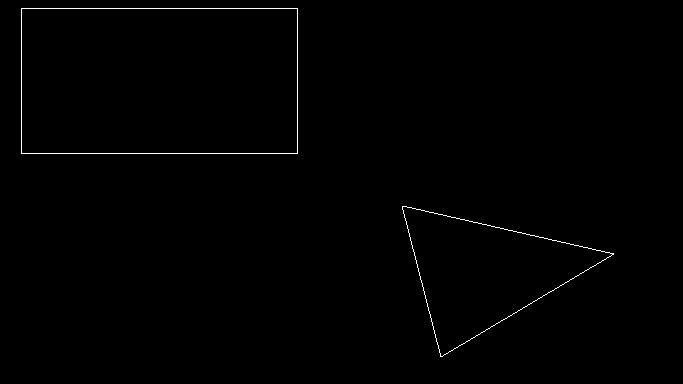
\includegraphics[width=0.9\columnwidth]{figures.jpg}
            \caption{Random input sample with shapes to the PHT.}
            \label{fig:fig1}
        \end{figure}
        \begin{figure}
            \centering
            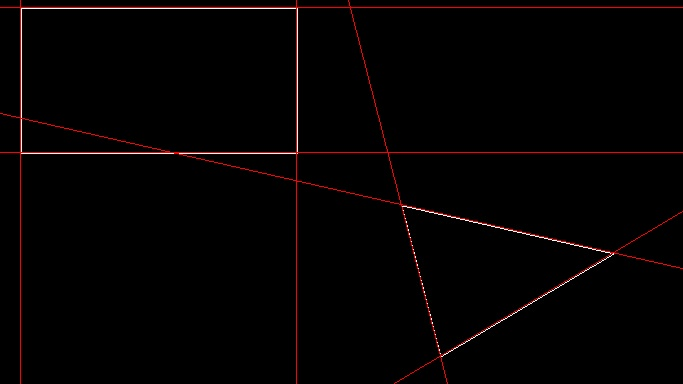
\includegraphics[width=0.9\columnwidth]{figures-HT.jpg}
            \caption{Output of the PHT applied to Figure \ref{fig:fig1}.}
            \label{fig:fig2}
            
        \end{figure}

    \end{itemize}

    To summarize, this analysis demonstrates that OMP implementations consistently delivered higher performance due to their ability to efficiently manage shared resources and minimize communication overhead, particularly compared to the MPI implementations. This underscores the critical importance of aligning and optimizing the chosen parallelization strategy with the specific computational characteristics of the algorithms to maximize efficiency.
    
\bibliographystyle{IEEEtran}
\bibliography{references}

\twocolumn[
\begin{@twocolumnfalse}
    \vspace*{\fill}
    \section*{\centering Appendix: Performance Charts}
    \label{sec::appendix}
    \vspace*{\fill}

    \begin{figure*}[htbp]
        \centering
        \caption{Efficiency matrices for each combination of image, HT version and parallelism and PBS properties.}
        \includegraphics[width=0.70\textwidth]{heatmap1.png}
    \end{figure*}
\end{@twocolumnfalse}

    \begin{figure*}[htbp]
        \centering
        \caption{Efficiency matrices for each combination of image, HT version and parallelism and PBS properties.}
        \includegraphics[width=0.75\textwidth]{heatmap2.png}
    \end{figure*}
    \begin{figure*}[htbp]
        \centering
        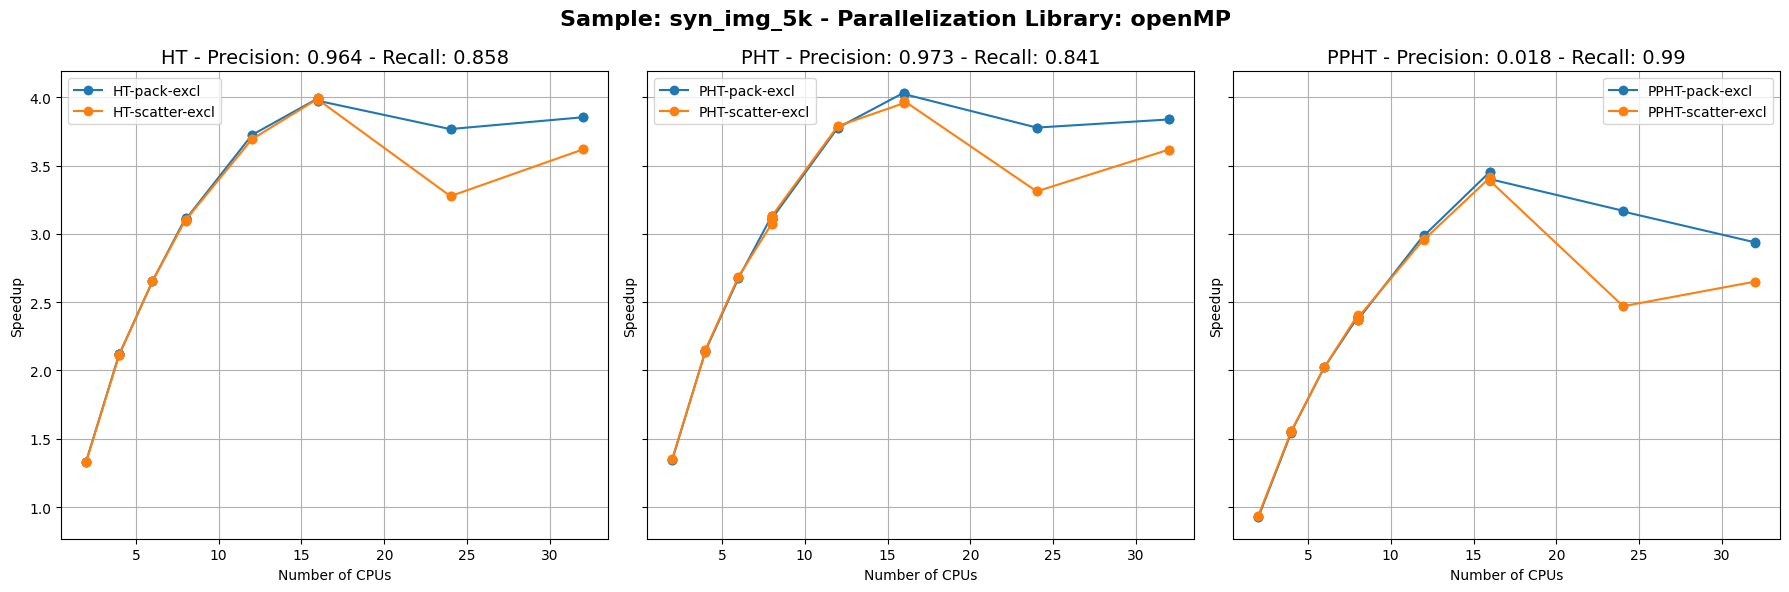
\includegraphics[width=0.75\textwidth]{lc-syn_img_5k-openMP.png}
    \end{figure*}
    \begin{figure*}[htbp]
        \caption{Speedup line charts for OMP and MPI.}
    
        \centering
        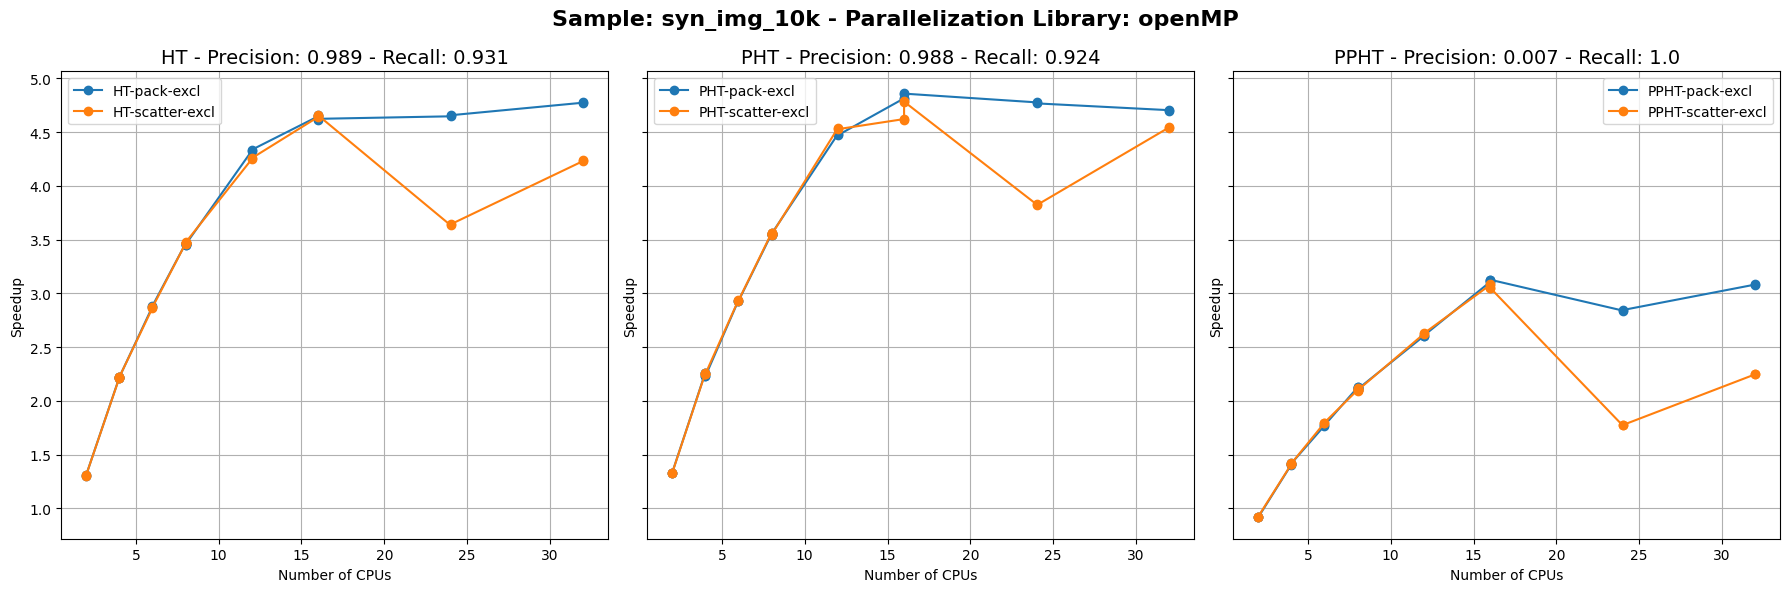
\includegraphics[width=0.75\textwidth]{lc-syn_img_10k-openMP.png}
        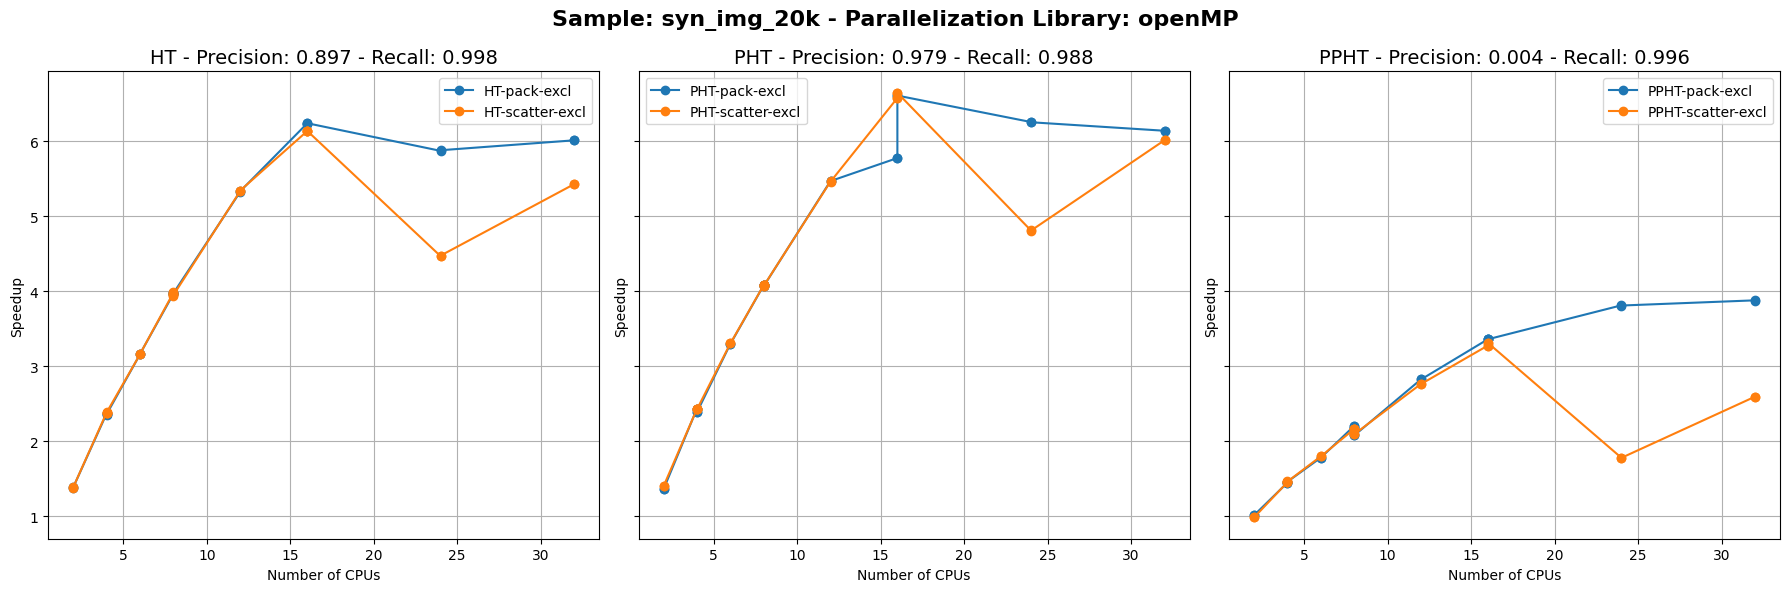
\includegraphics[width=0.75\textwidth]{lc-syn_img_20k-openMP.png}
        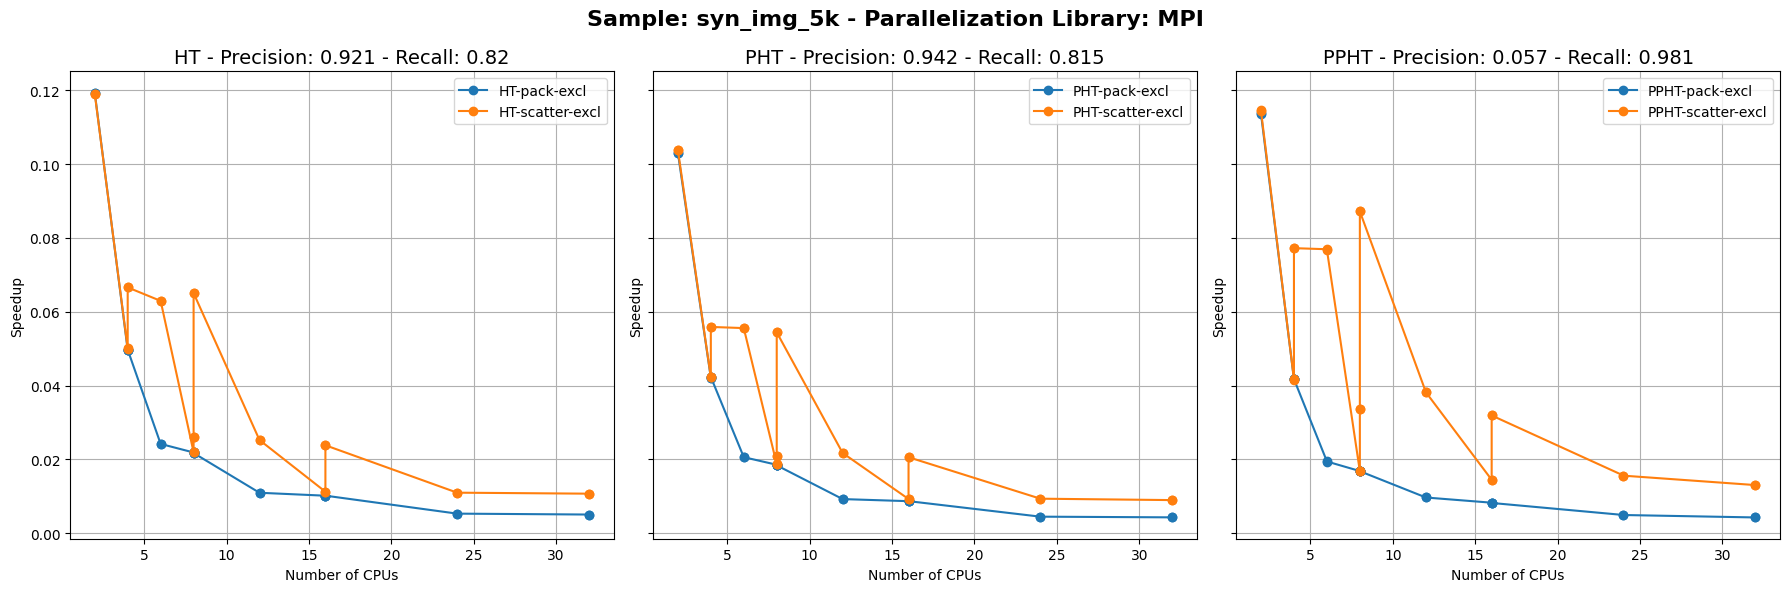
\includegraphics[width=0.75\textwidth]{lc-syn_img_5k-MPI.png}
        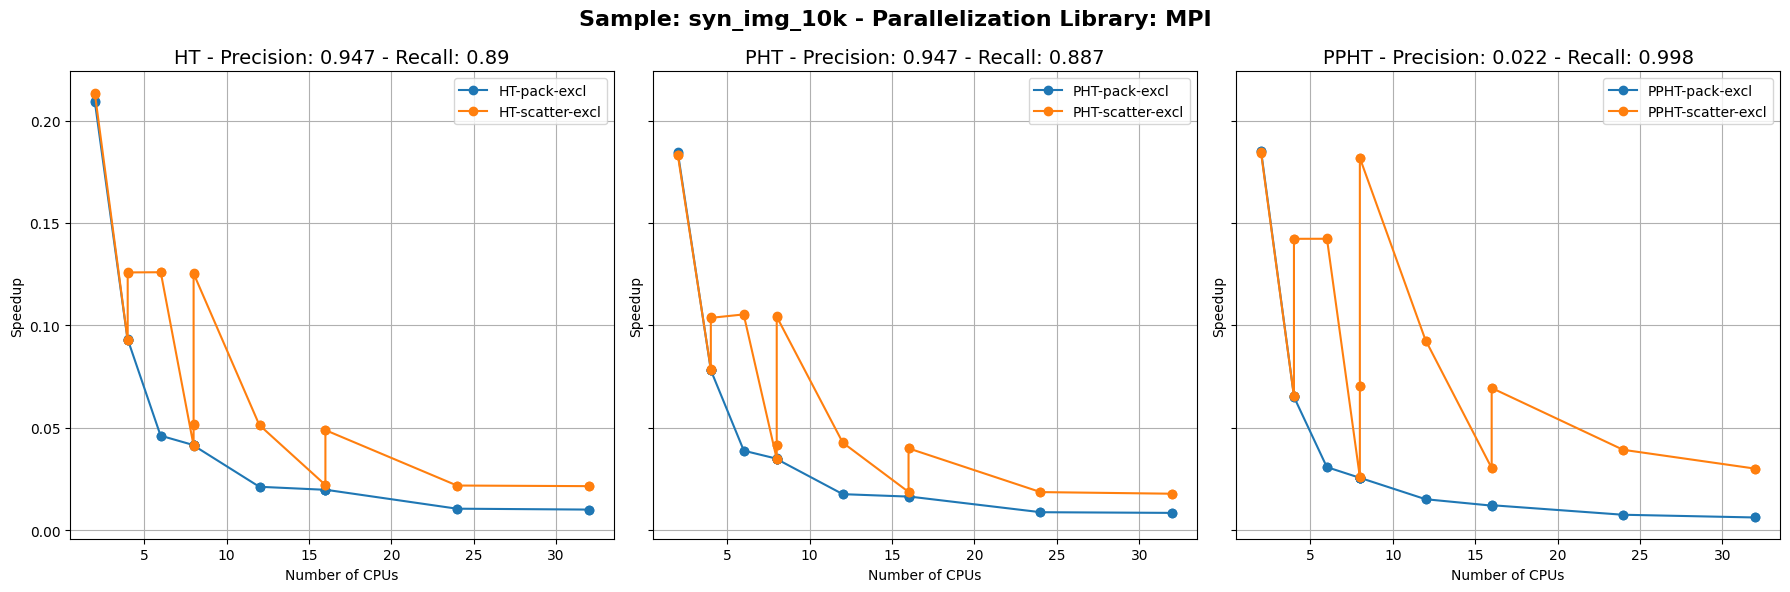
\includegraphics[width=0.75\textwidth]{lc-syn_img_10k-MPI.png}
        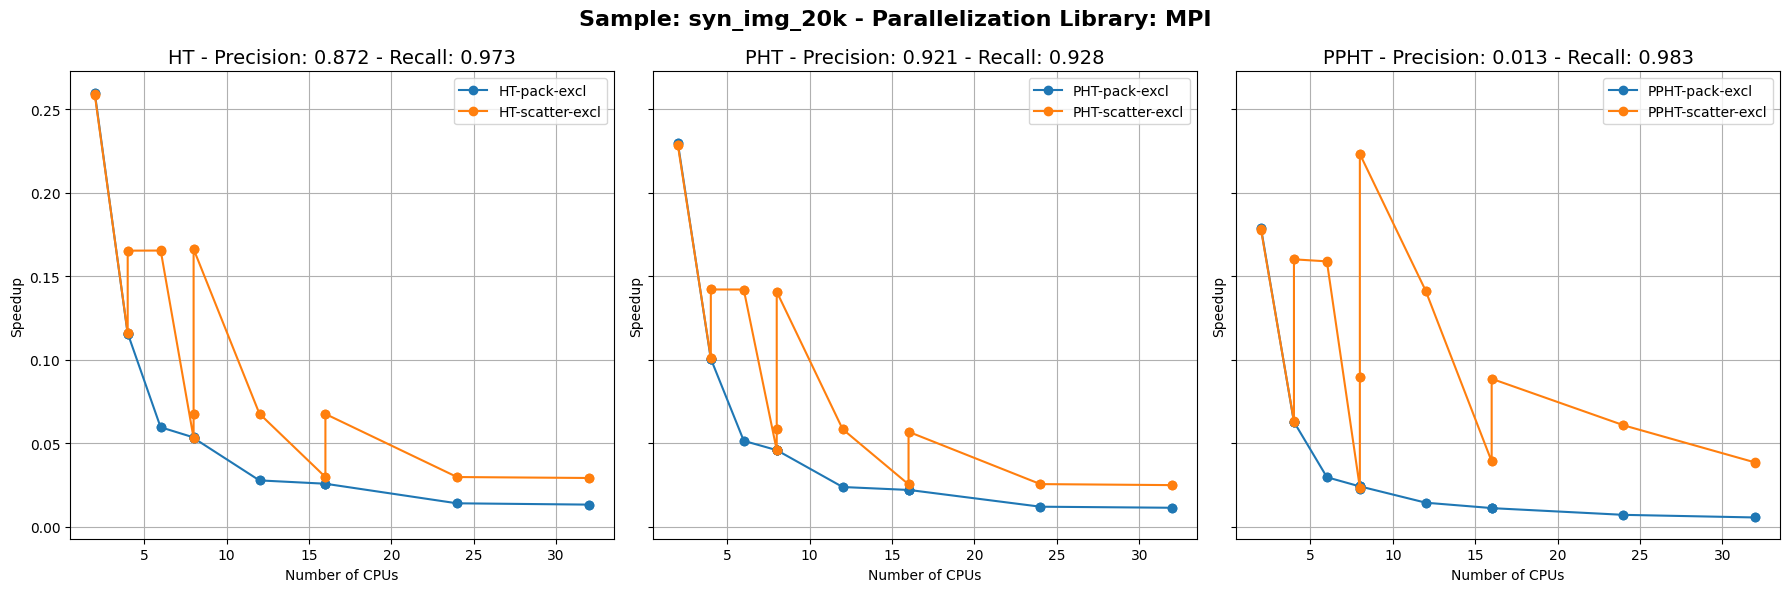
\includegraphics[width=0.75\textwidth]{lc-syn_img_20k-MPI.png}
        
    \end{figure*}
    \begin{figure*}
    
        \caption{Speedup line charts Hybrid parallelism.}
        
        \centering
        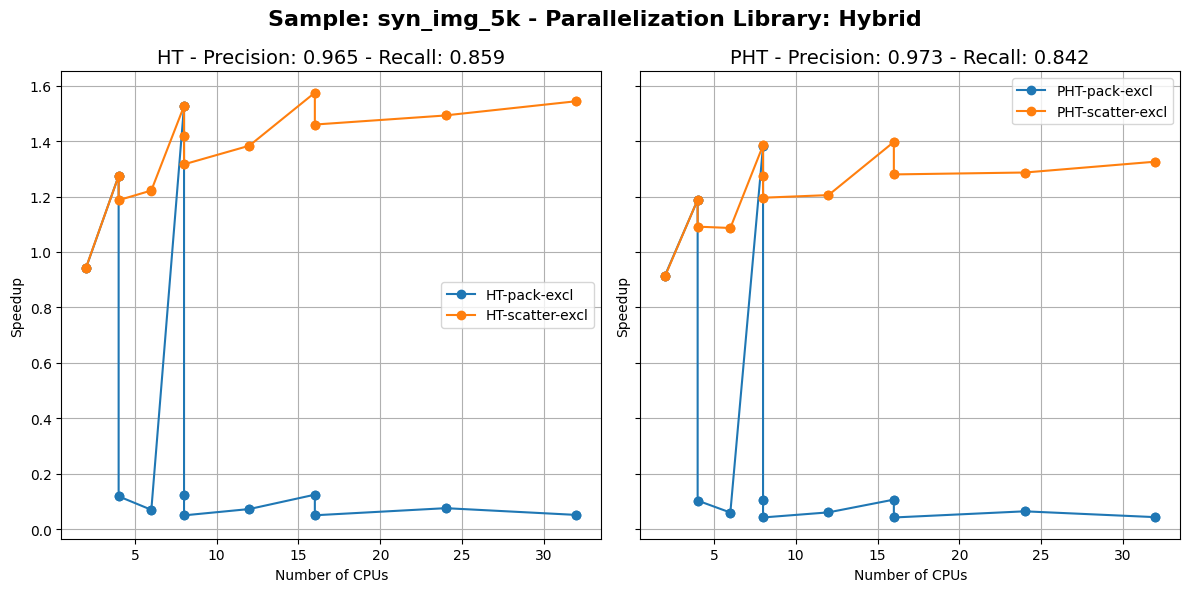
\includegraphics[width=0.6\textwidth]{lc-syn_img_5k-Hybrid.png}
    
        \centering
        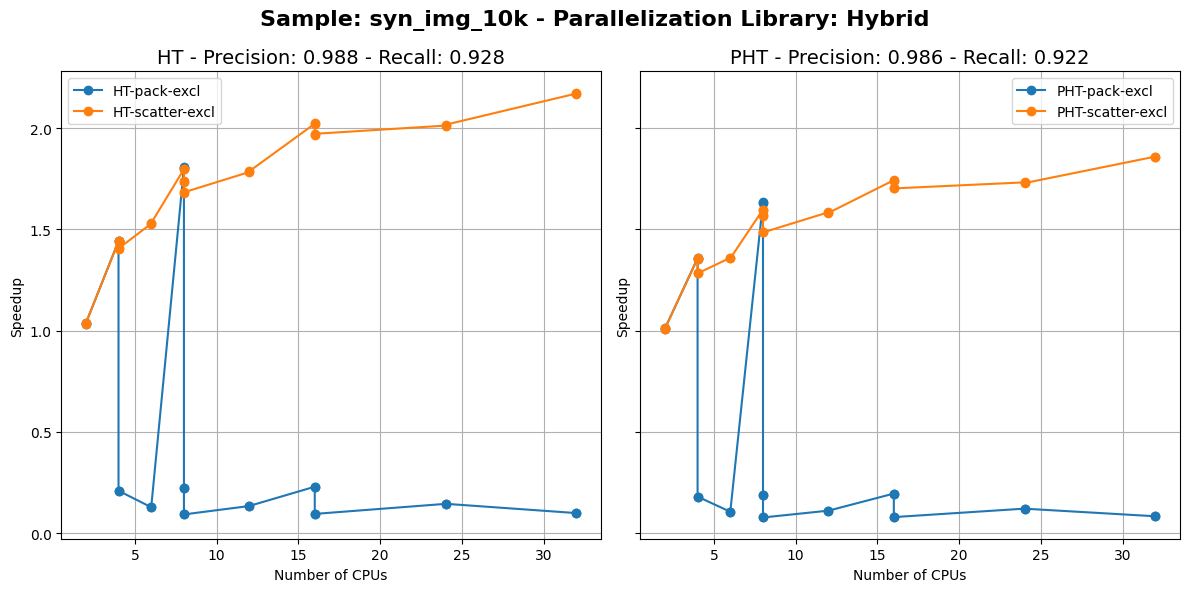
\includegraphics[width=0.6\textwidth]{lc-syn_img_10k-Hybrid.png}
        
        \centering
        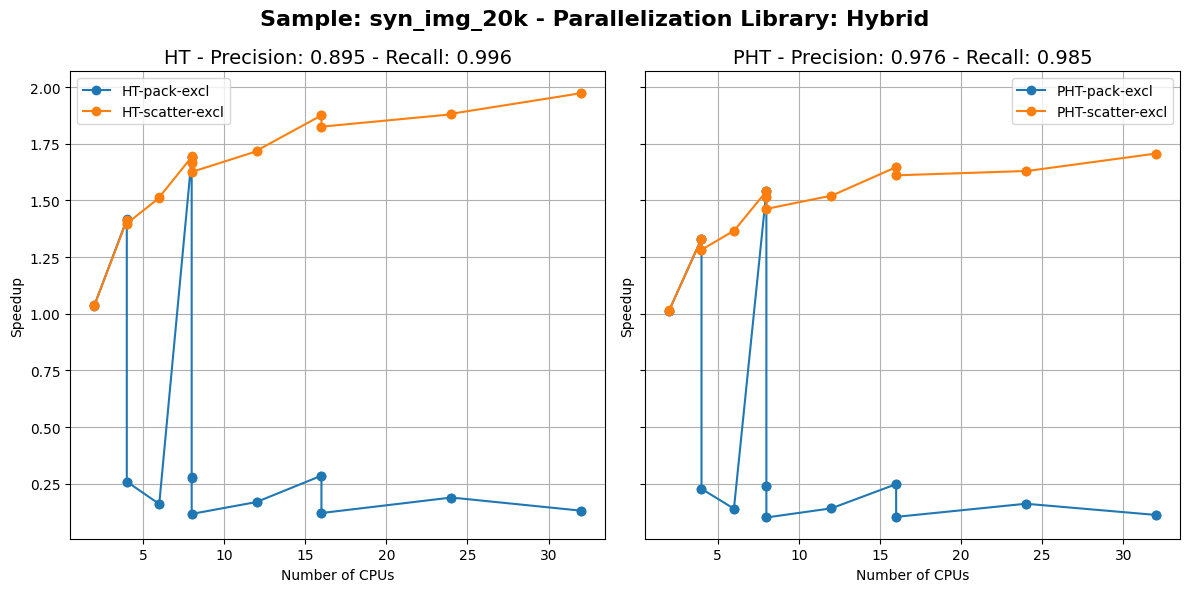
\includegraphics[width=0.6\textwidth]{lc-syn_img_20k-Hybrid.png}
    \end{figure*} 


\end{document}
